% Automatically generated figure inventory for task2.

\begin{figure}[H]
\centering
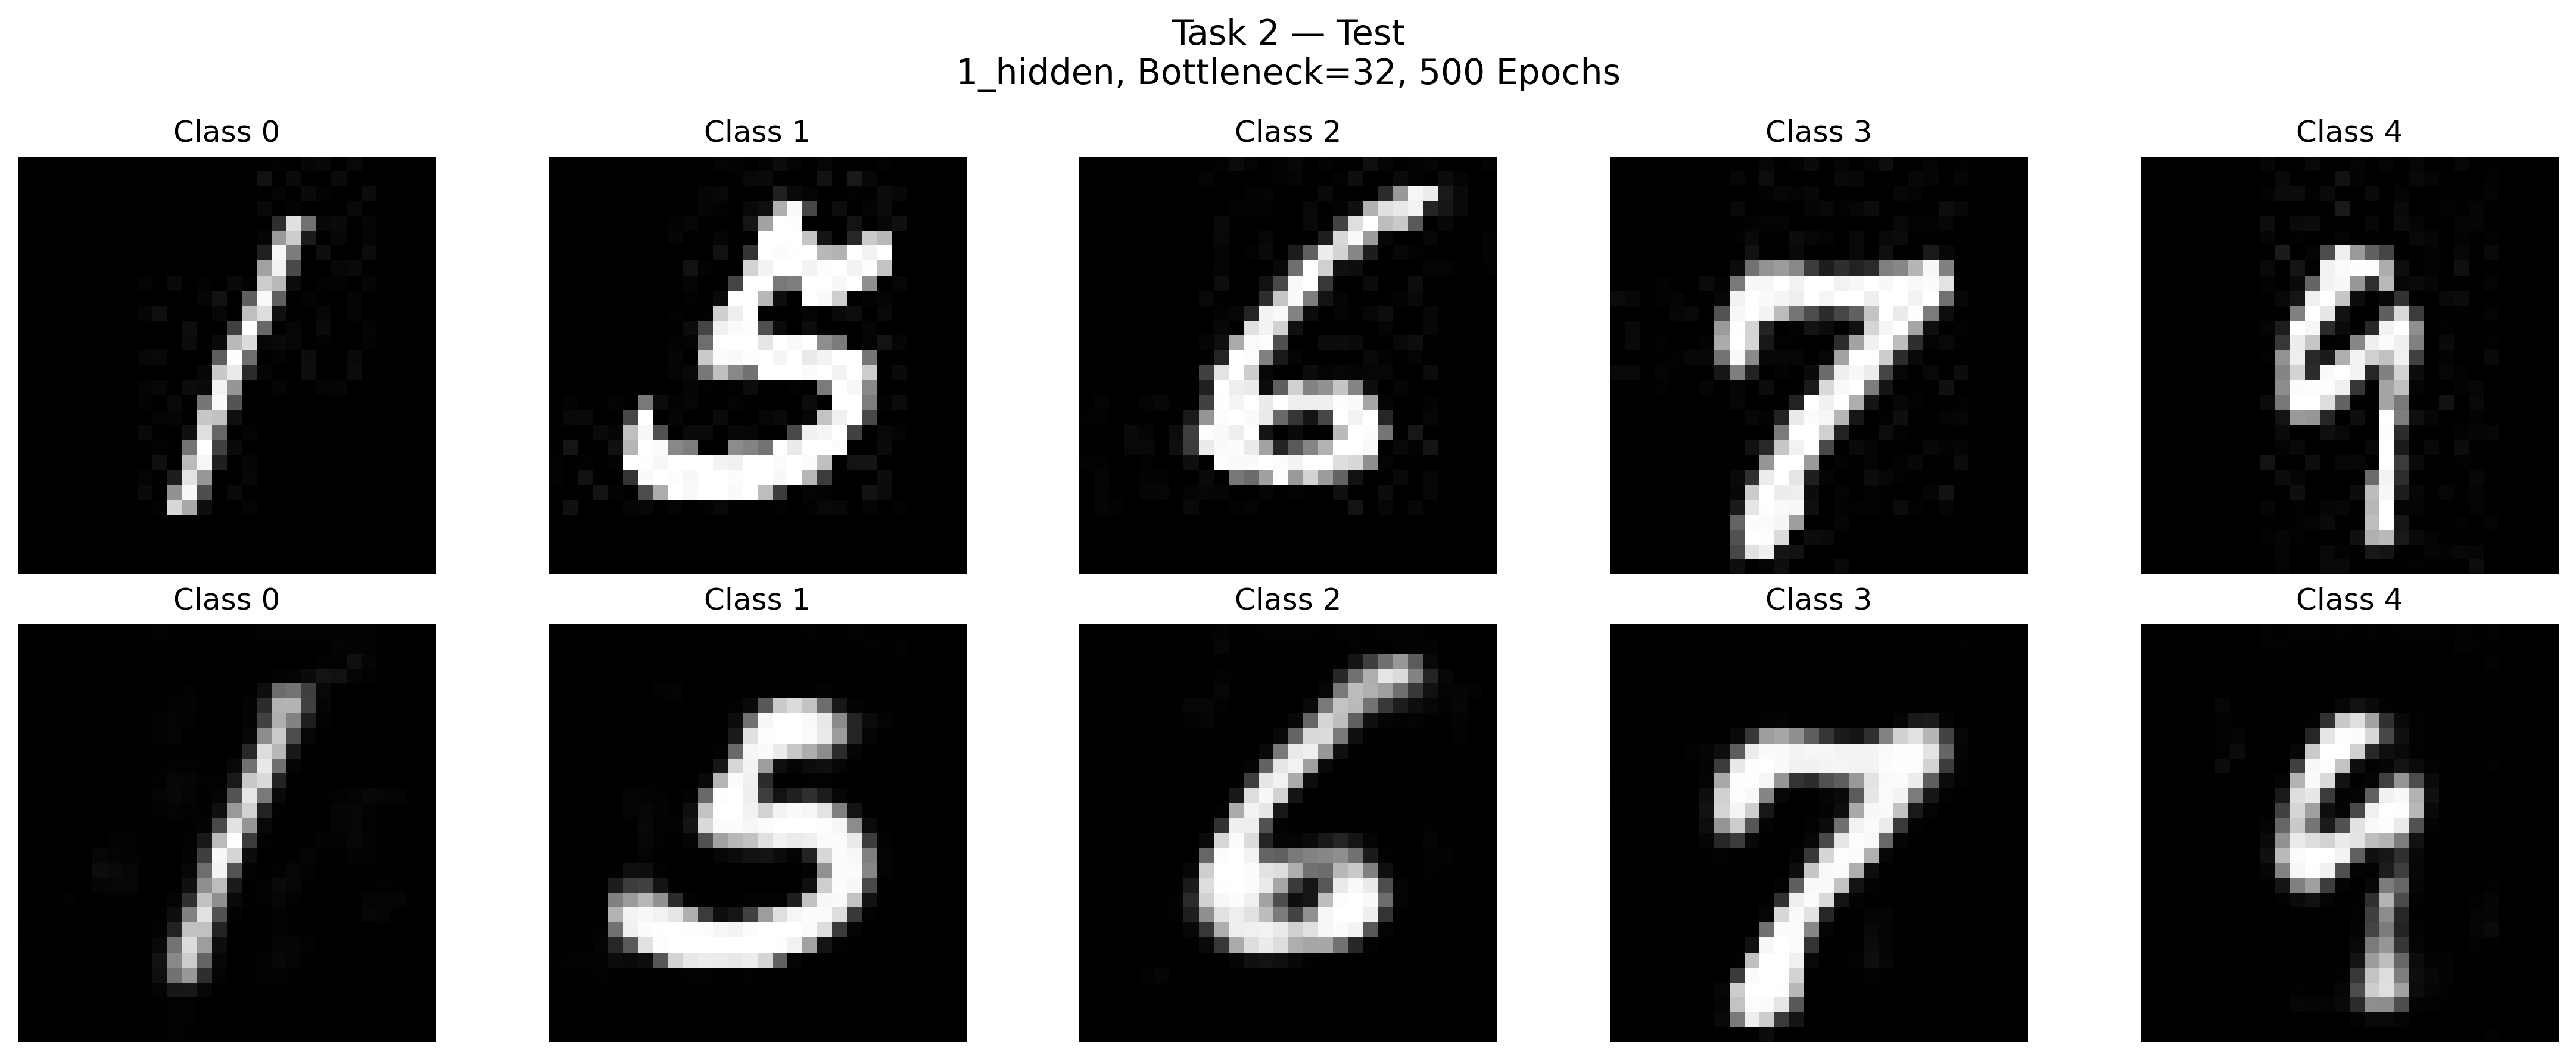
\includegraphics[width=0.96\linewidth,height=0.48\textheight,keepaspectratio]{figures/task2/model_reconstruction_visualization_500/test_1_hidden_bottleneck_32_500epochs.png}
\caption{Autoencoder reconstruction visualization: test 1 hidden with bottleneck of 32 neurons.}
\label{fig:task2_1}
\end{figure}

\begin{figure}[H]
\centering
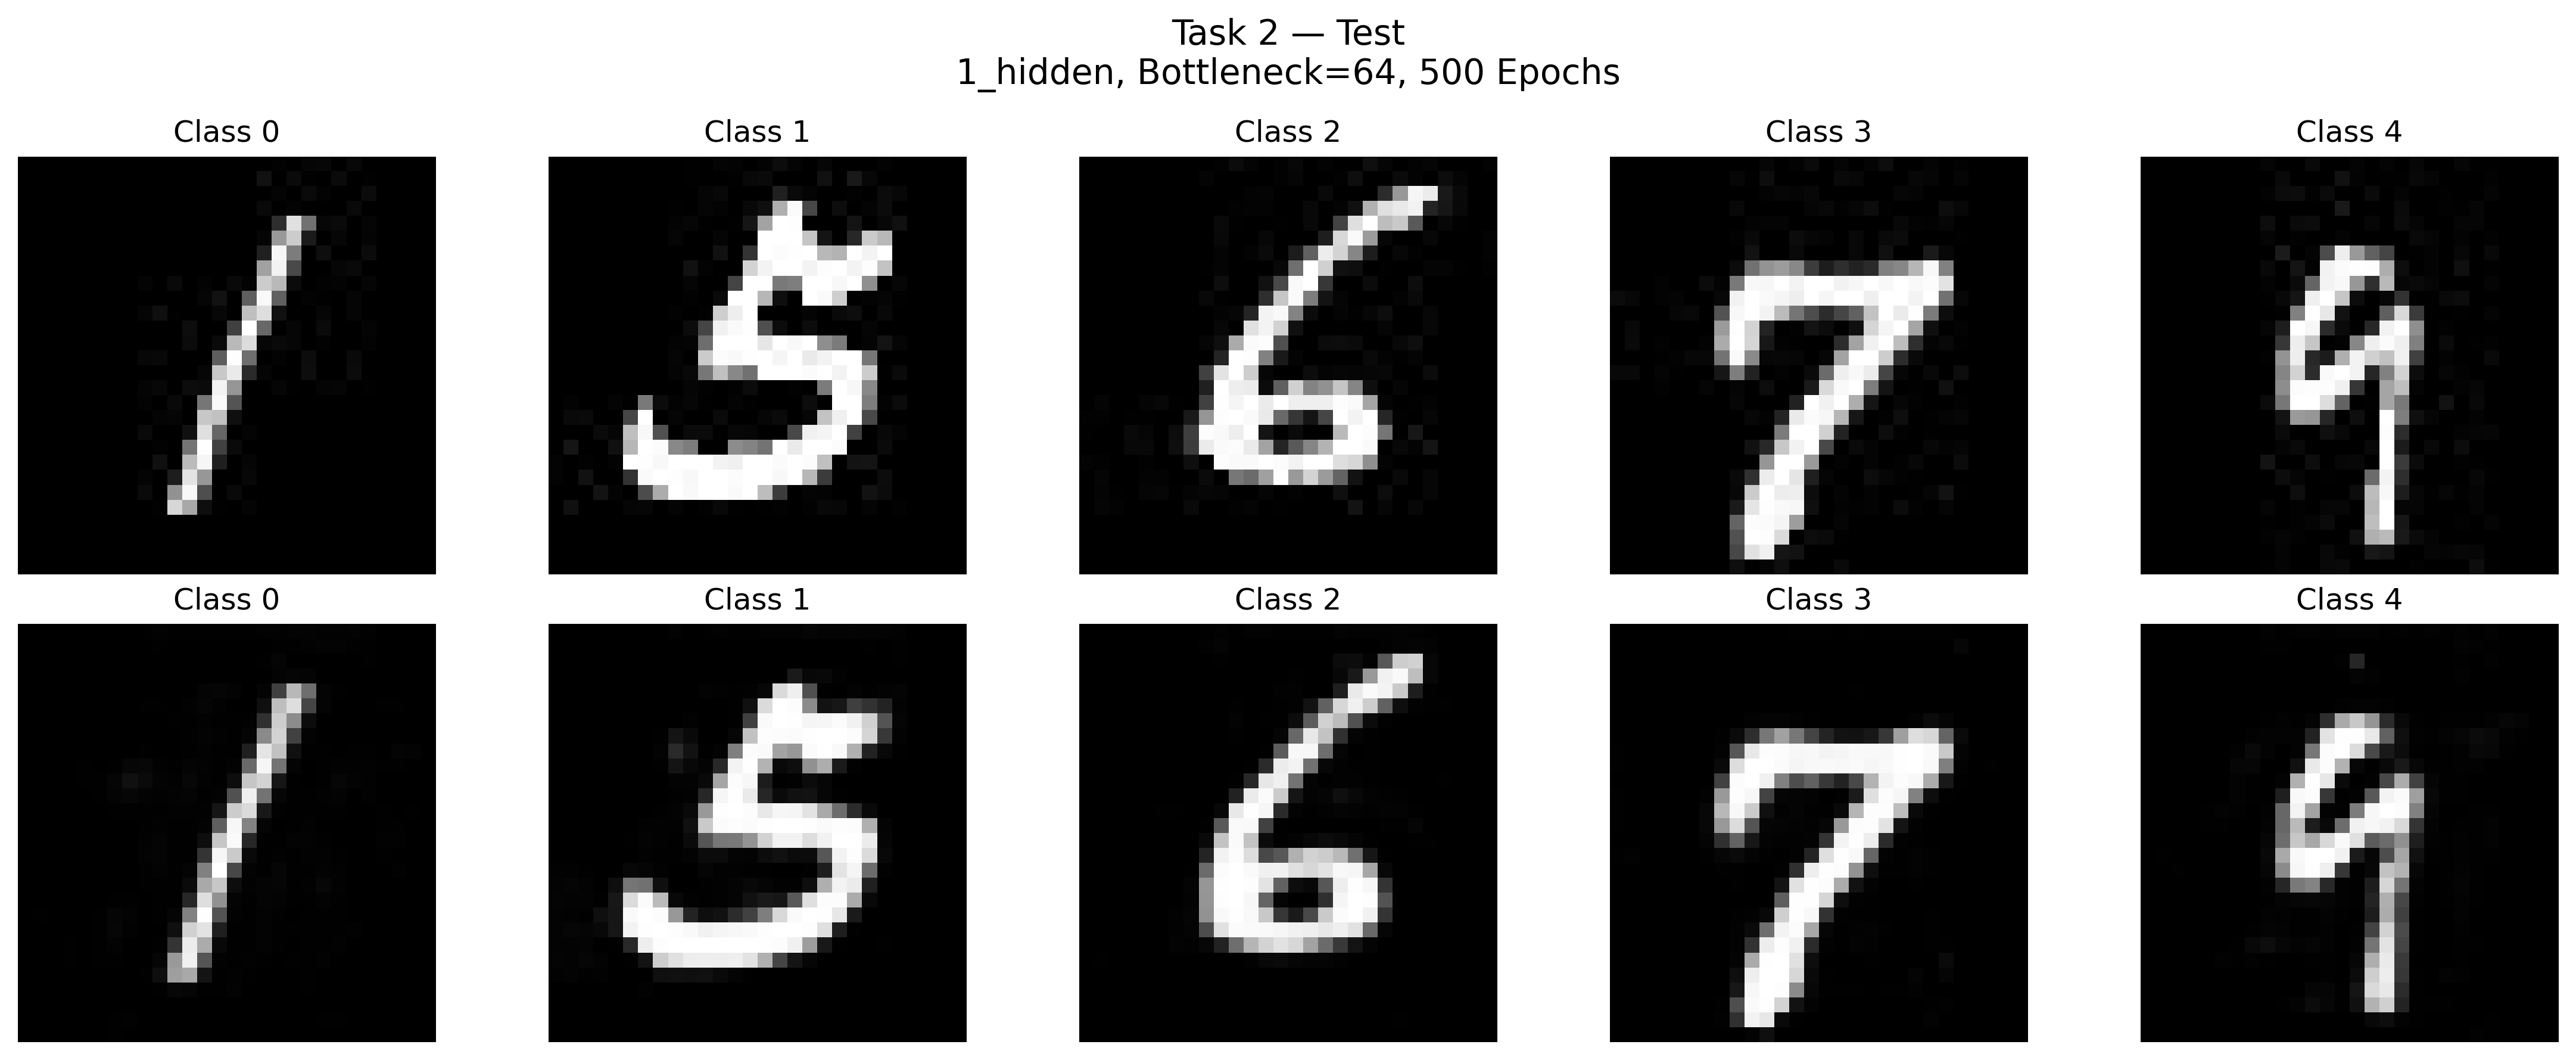
\includegraphics[width=0.96\linewidth,height=0.48\textheight,keepaspectratio]{figures/task2/model_reconstruction_visualization_500/test_1_hidden_bottleneck_64_500epochs.png}
\caption{Autoencoder reconstruction visualization: test 1 hidden with bottleneck of 64 neurons.}
\label{fig:task2_2}
\end{figure}

\begin{figure}[H]
\centering
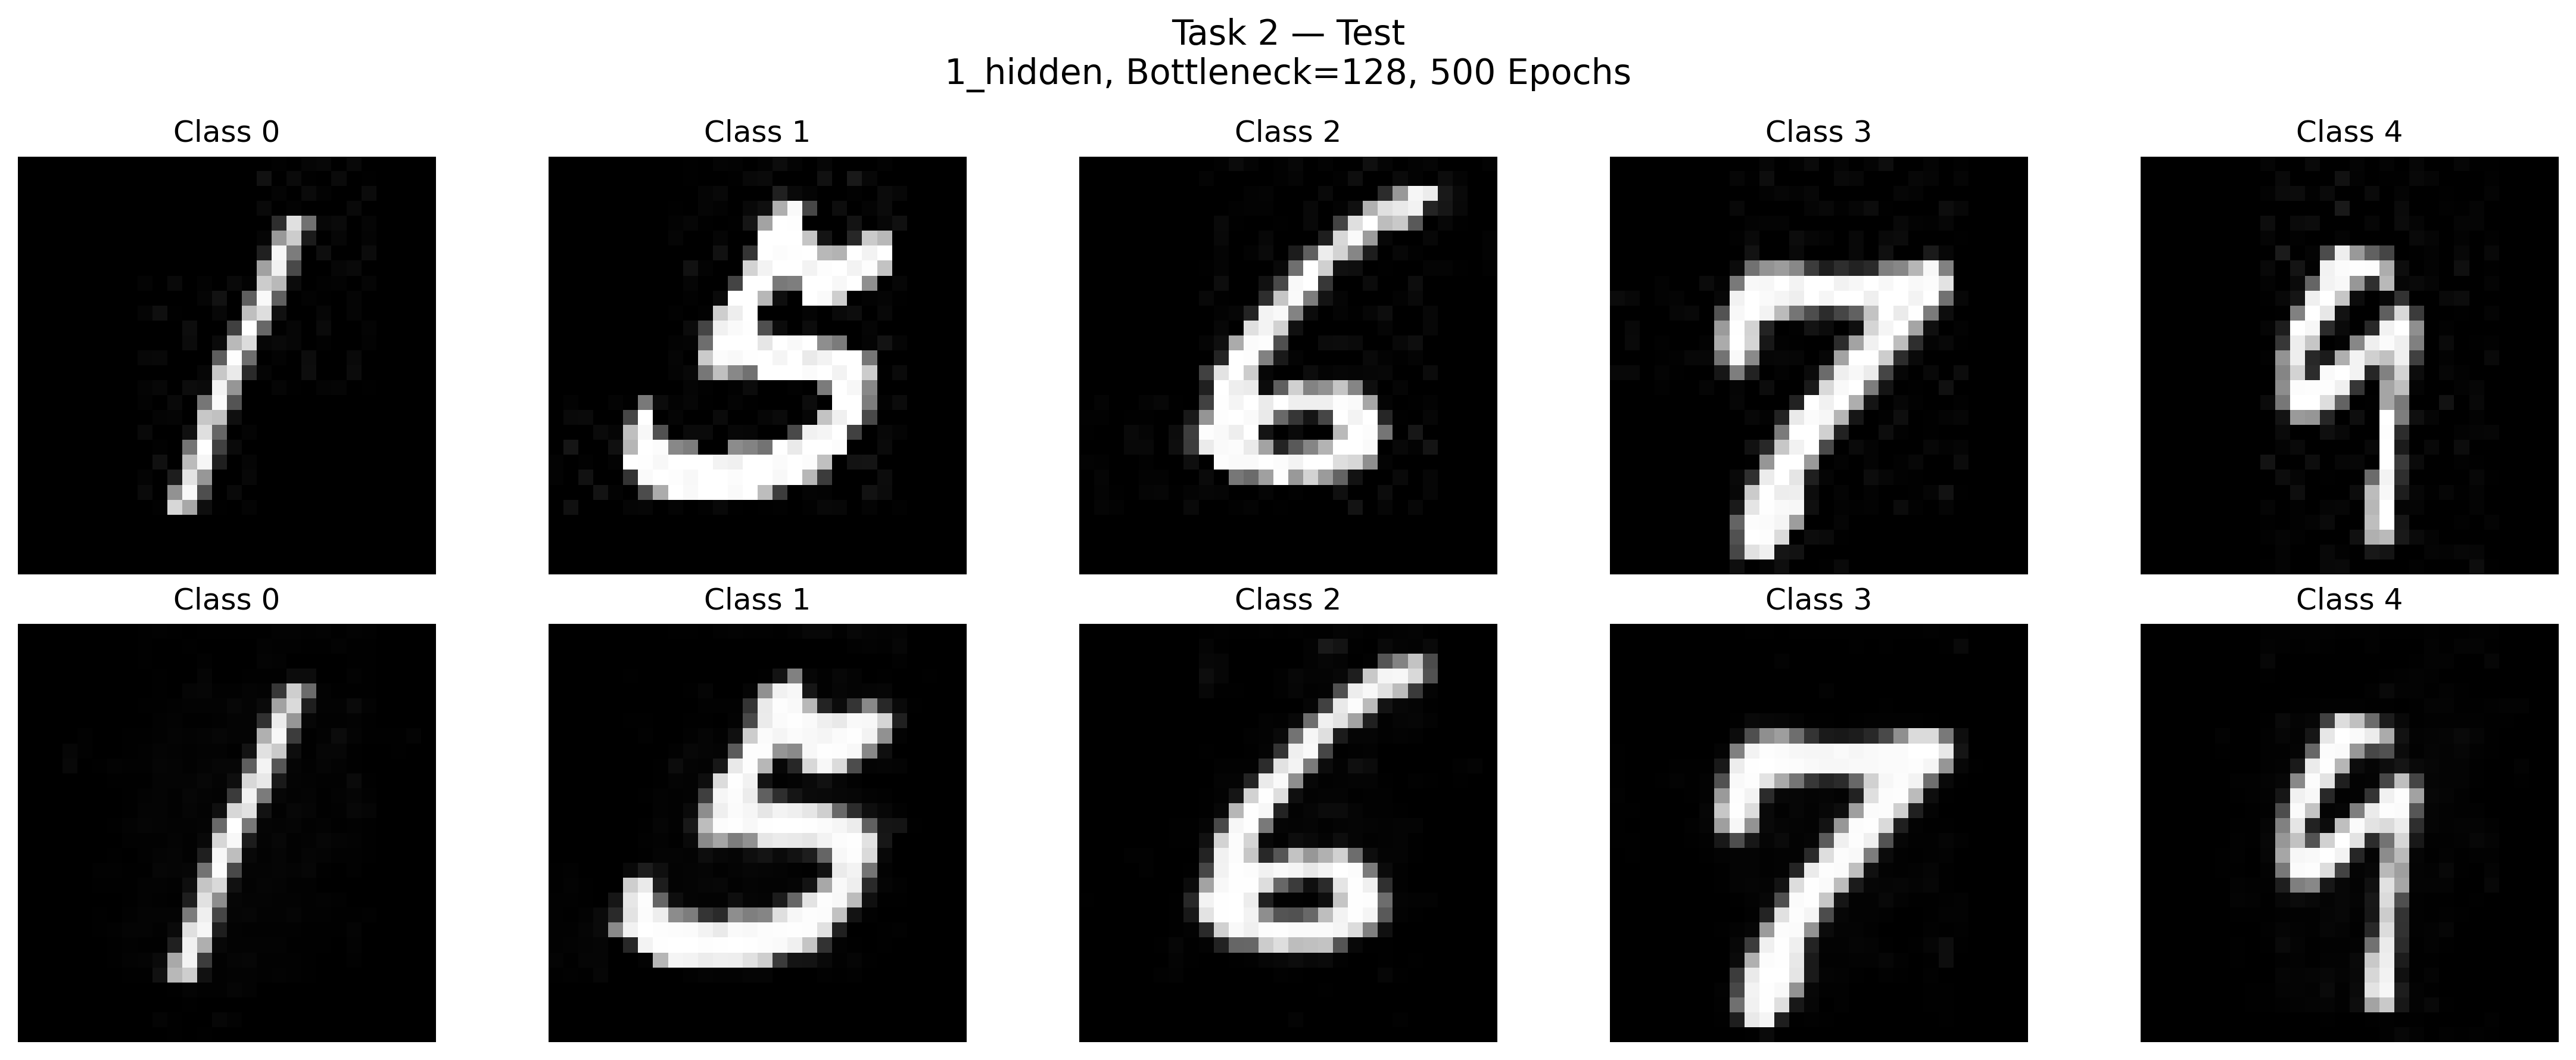
\includegraphics[width=0.96\linewidth,height=0.48\textheight,keepaspectratio]{figures/task2/model_reconstruction_visualization_500/test_1_hidden_bottleneck_128_500epochs.png}
\caption{Autoencoder reconstruction visualization: test 1 hidden with bottleneck of 128 neurons.}
\label{fig:task2_3}
\end{figure}

\begin{figure}[H]
\centering
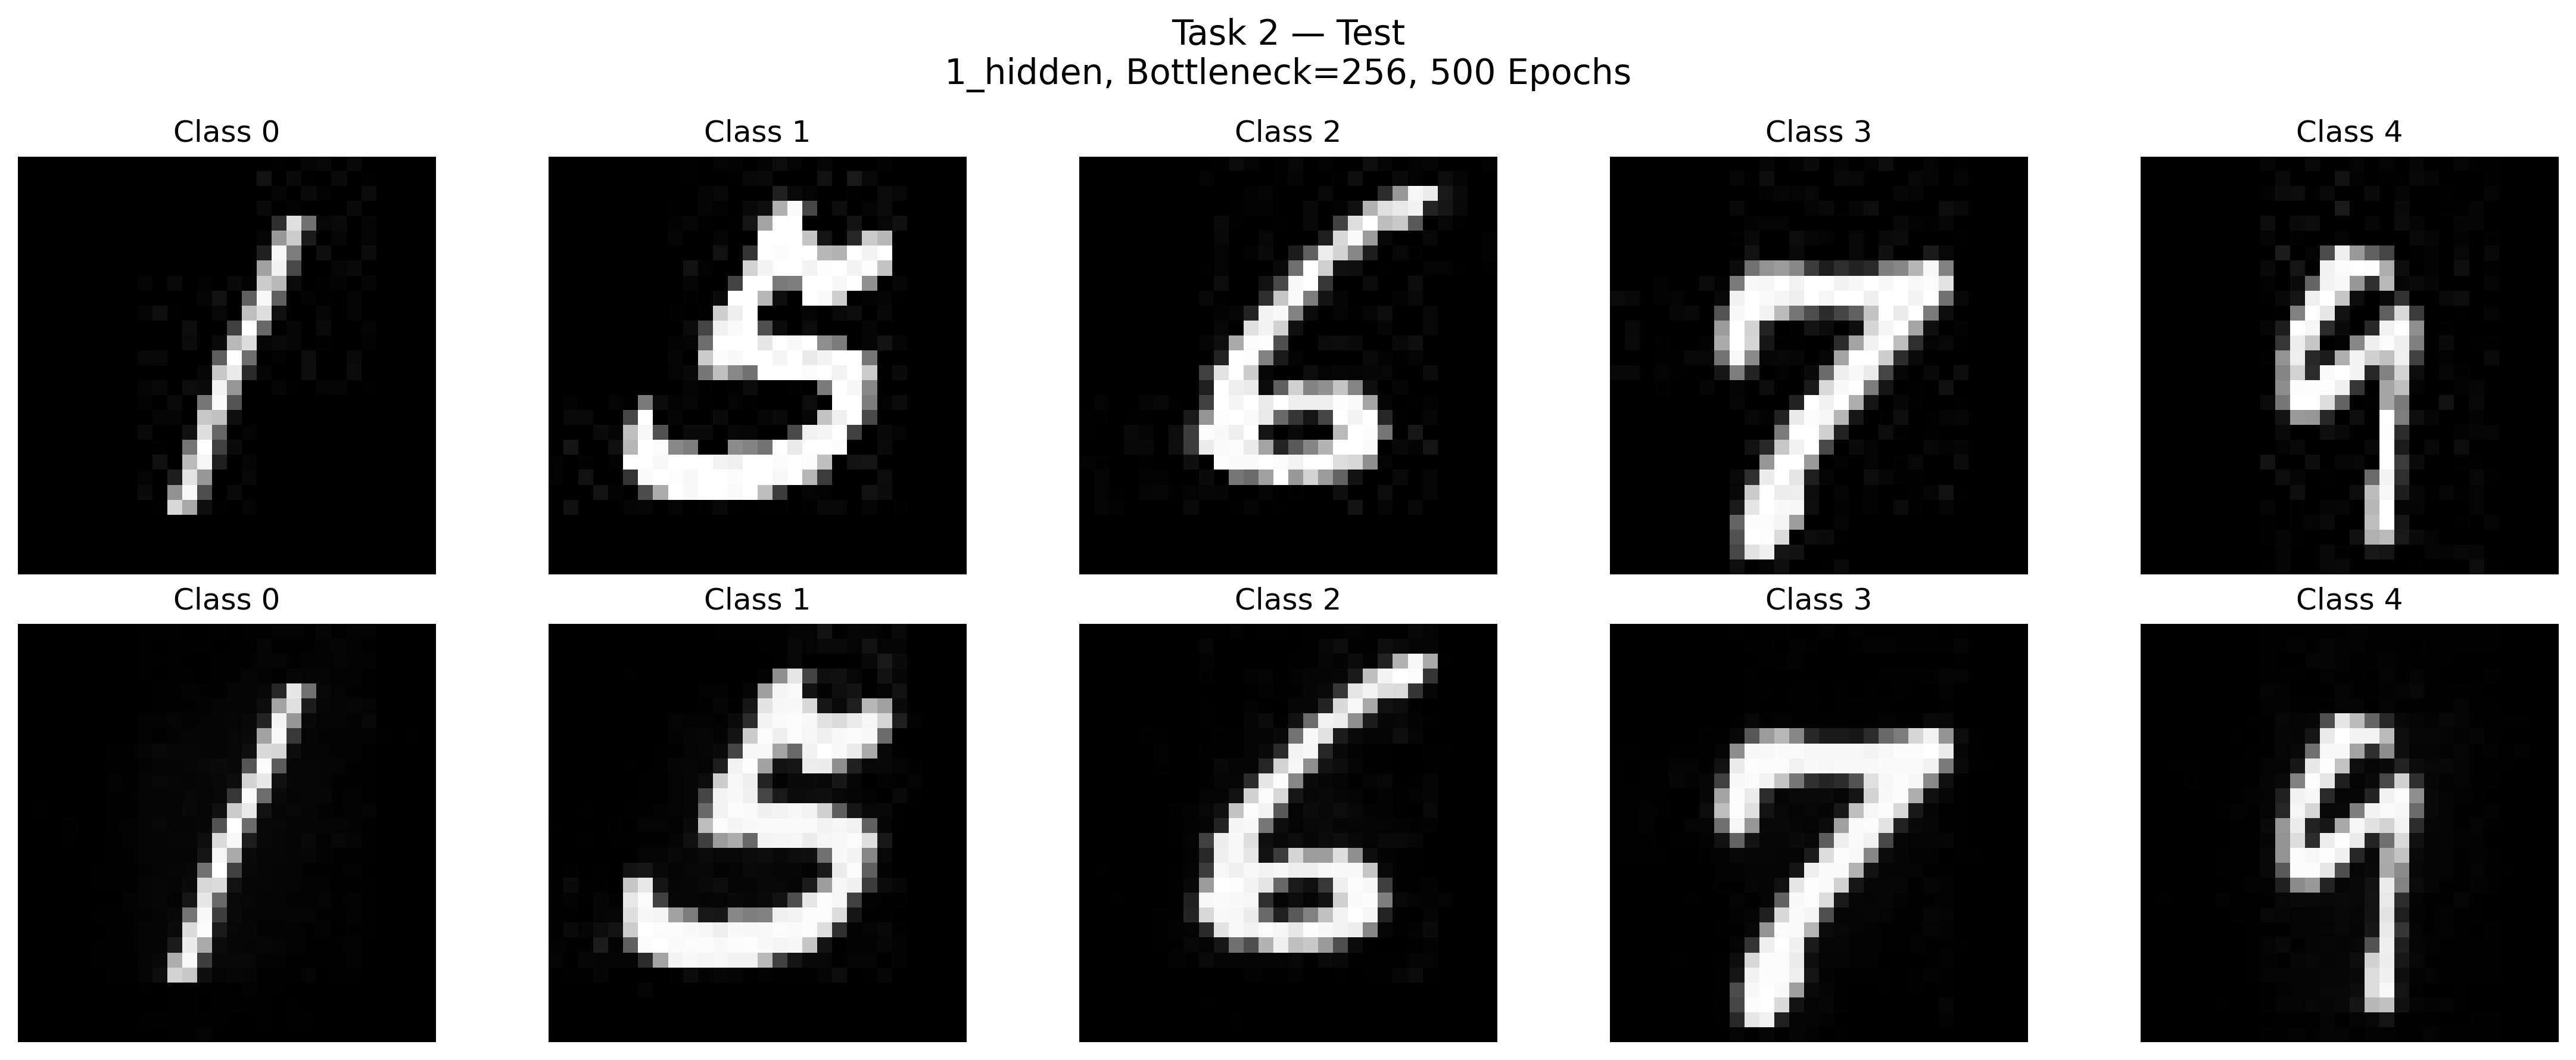
\includegraphics[width=0.96\linewidth,height=0.48\textheight,keepaspectratio]{figures/task2/model_reconstruction_visualization_500/test_1_hidden_bottleneck_256_500epochs.png}
\caption{Autoencoder reconstruction visualization: test 1 hidden with bottleneck of 256 neurons.}
\label{fig:task2_4}
\end{figure}

\begin{figure}[H]
\centering
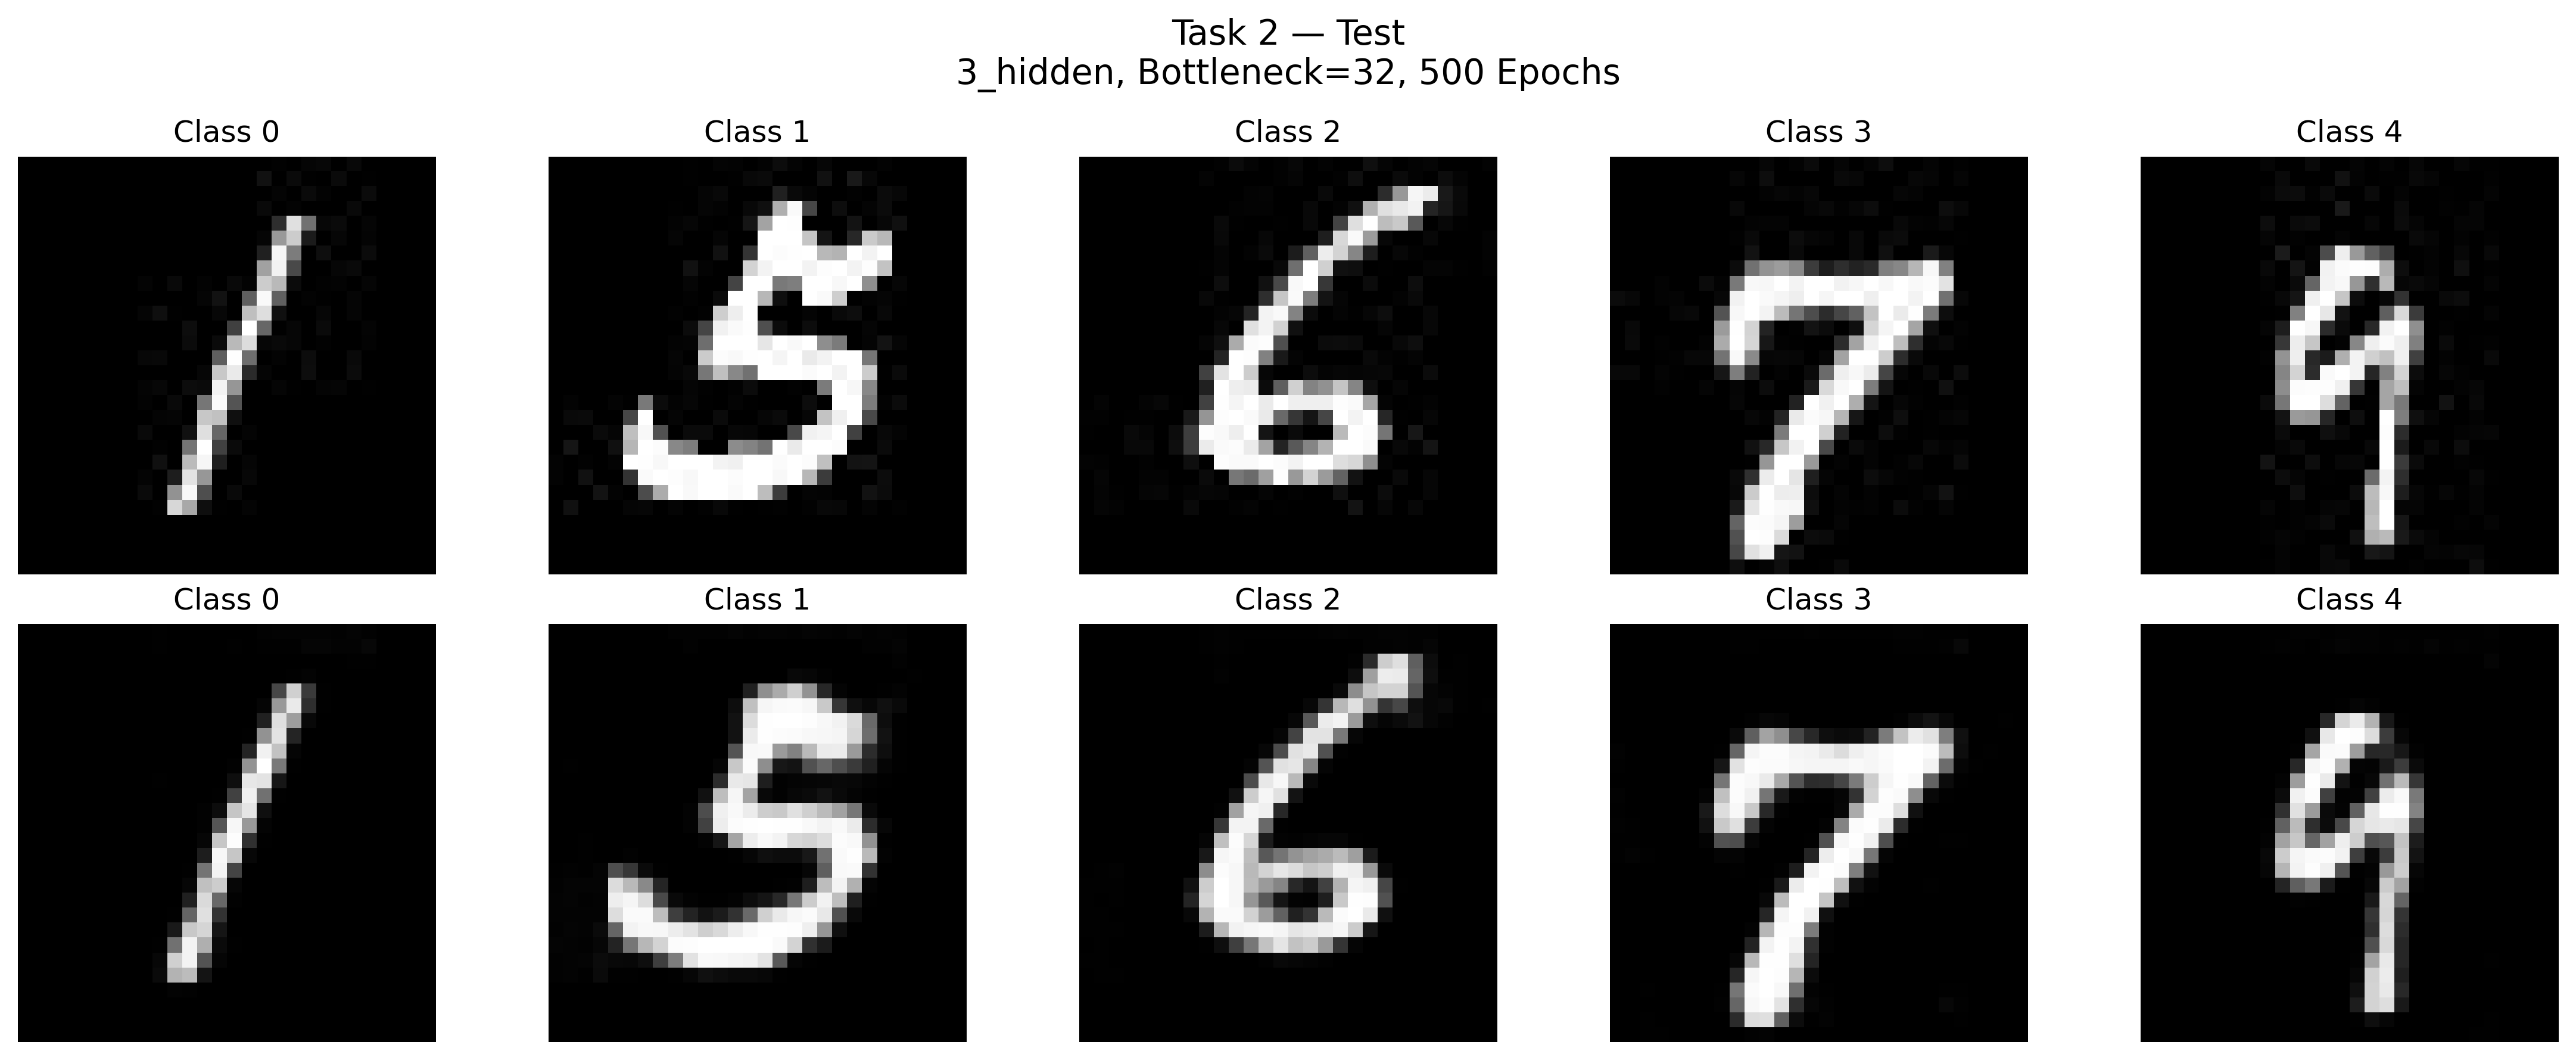
\includegraphics[width=0.96\linewidth,height=0.48\textheight,keepaspectratio]{figures/task2/model_reconstruction_visualization_500/test_3_hidden_bottleneck_32_500epochs.png}
\caption{Autoencoder reconstruction visualization: test 3 hidden with bottleneck of 32 neurons.}
\label{fig:task2_5}
\end{figure}

\begin{figure}[H]
\centering
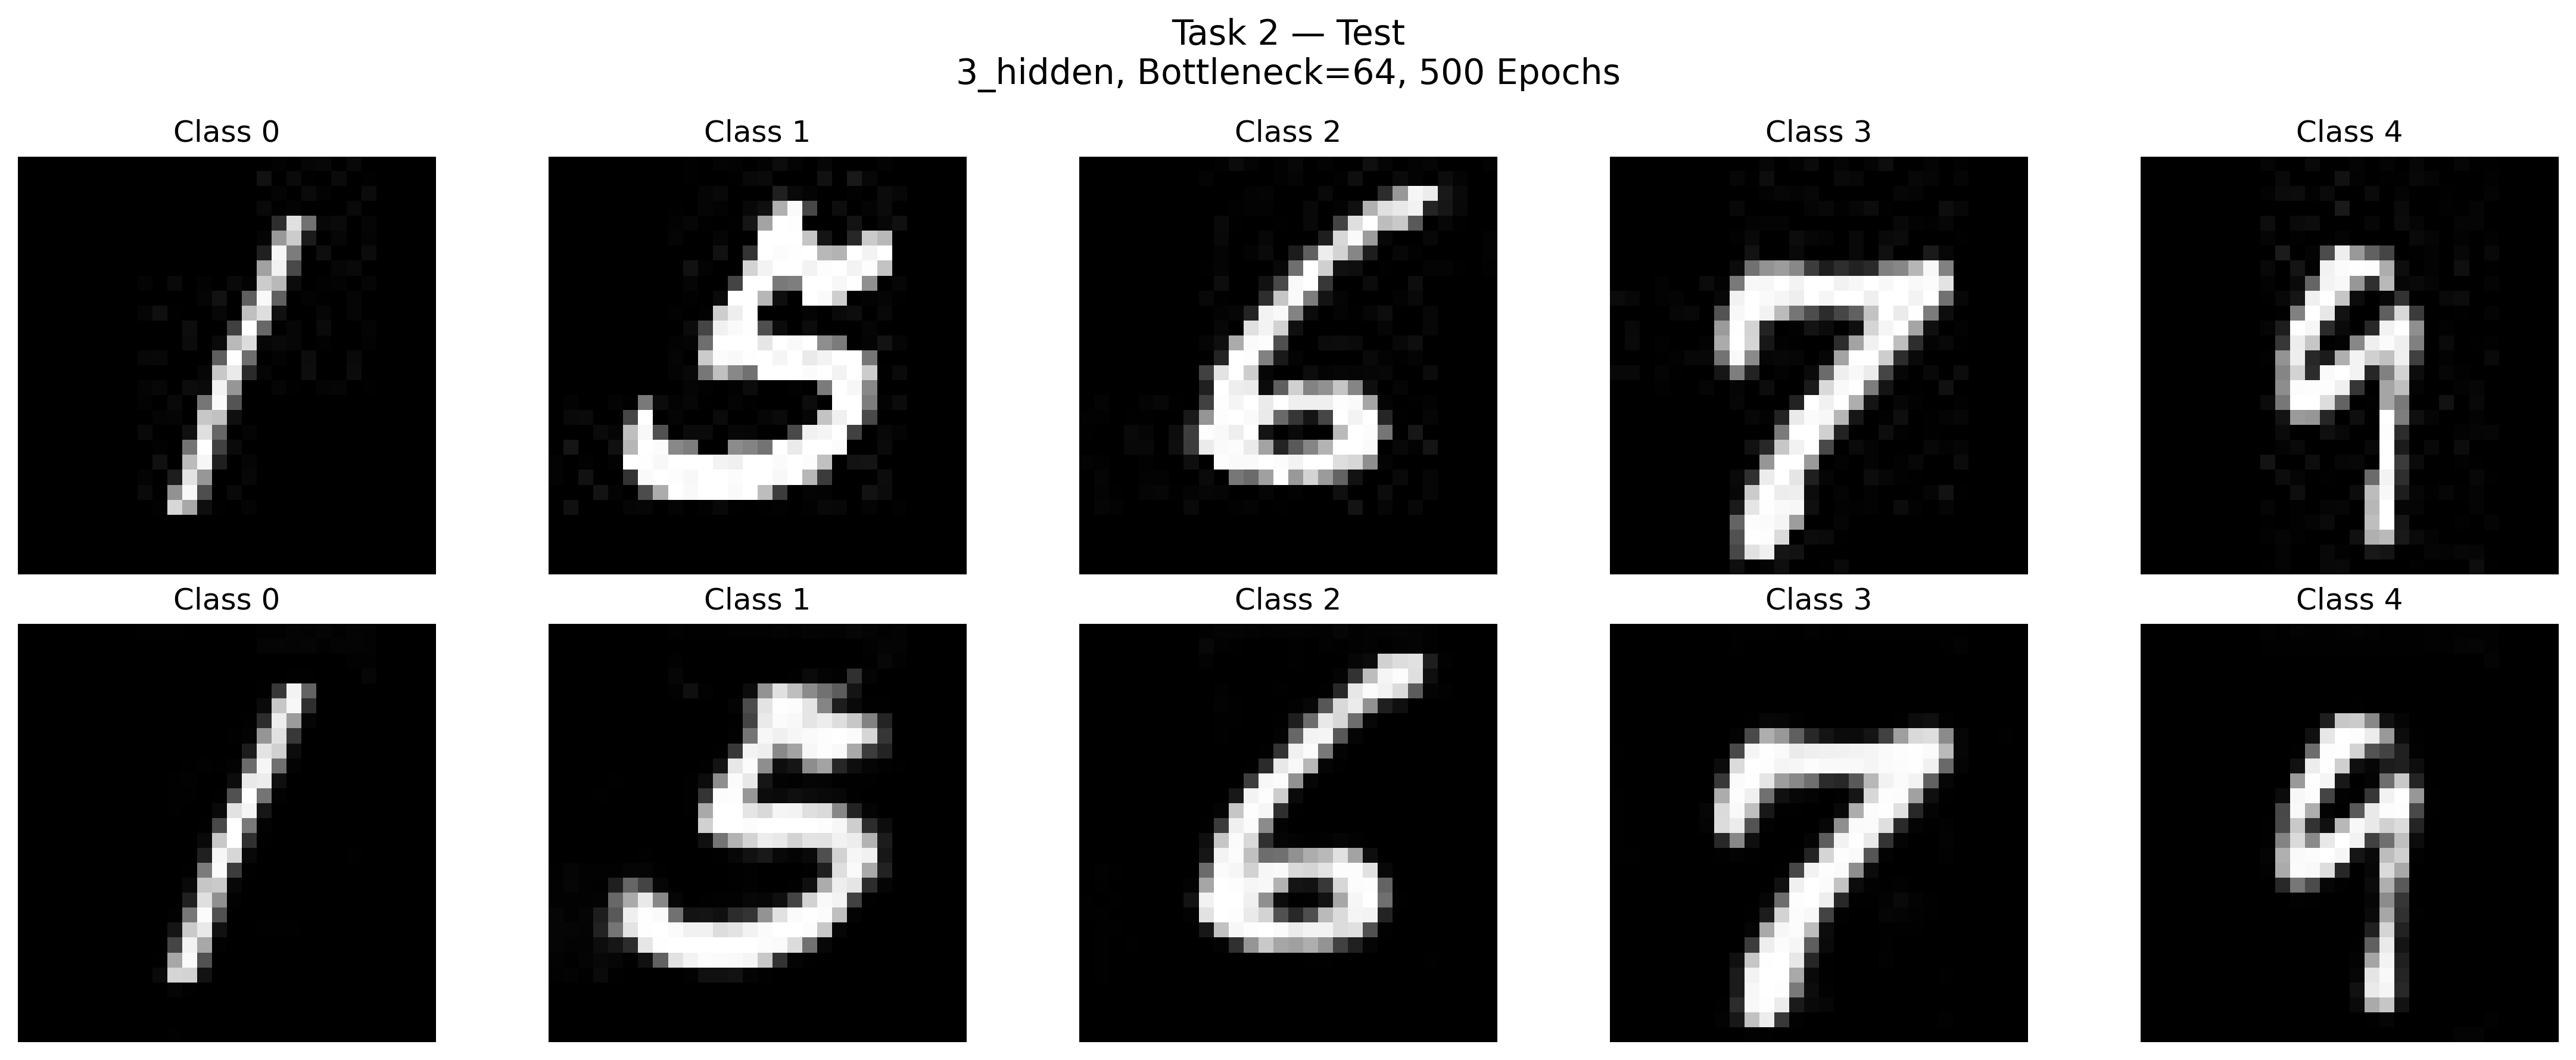
\includegraphics[width=0.96\linewidth,height=0.48\textheight,keepaspectratio]{figures/task2/model_reconstruction_visualization_500/test_3_hidden_bottleneck_64_500epochs.png}
\caption{Autoencoder reconstruction visualization: test 3 hidden with bottleneck of 64 neurons.}
\label{fig:task2_6}
\end{figure}

\begin{figure}[H]
\centering
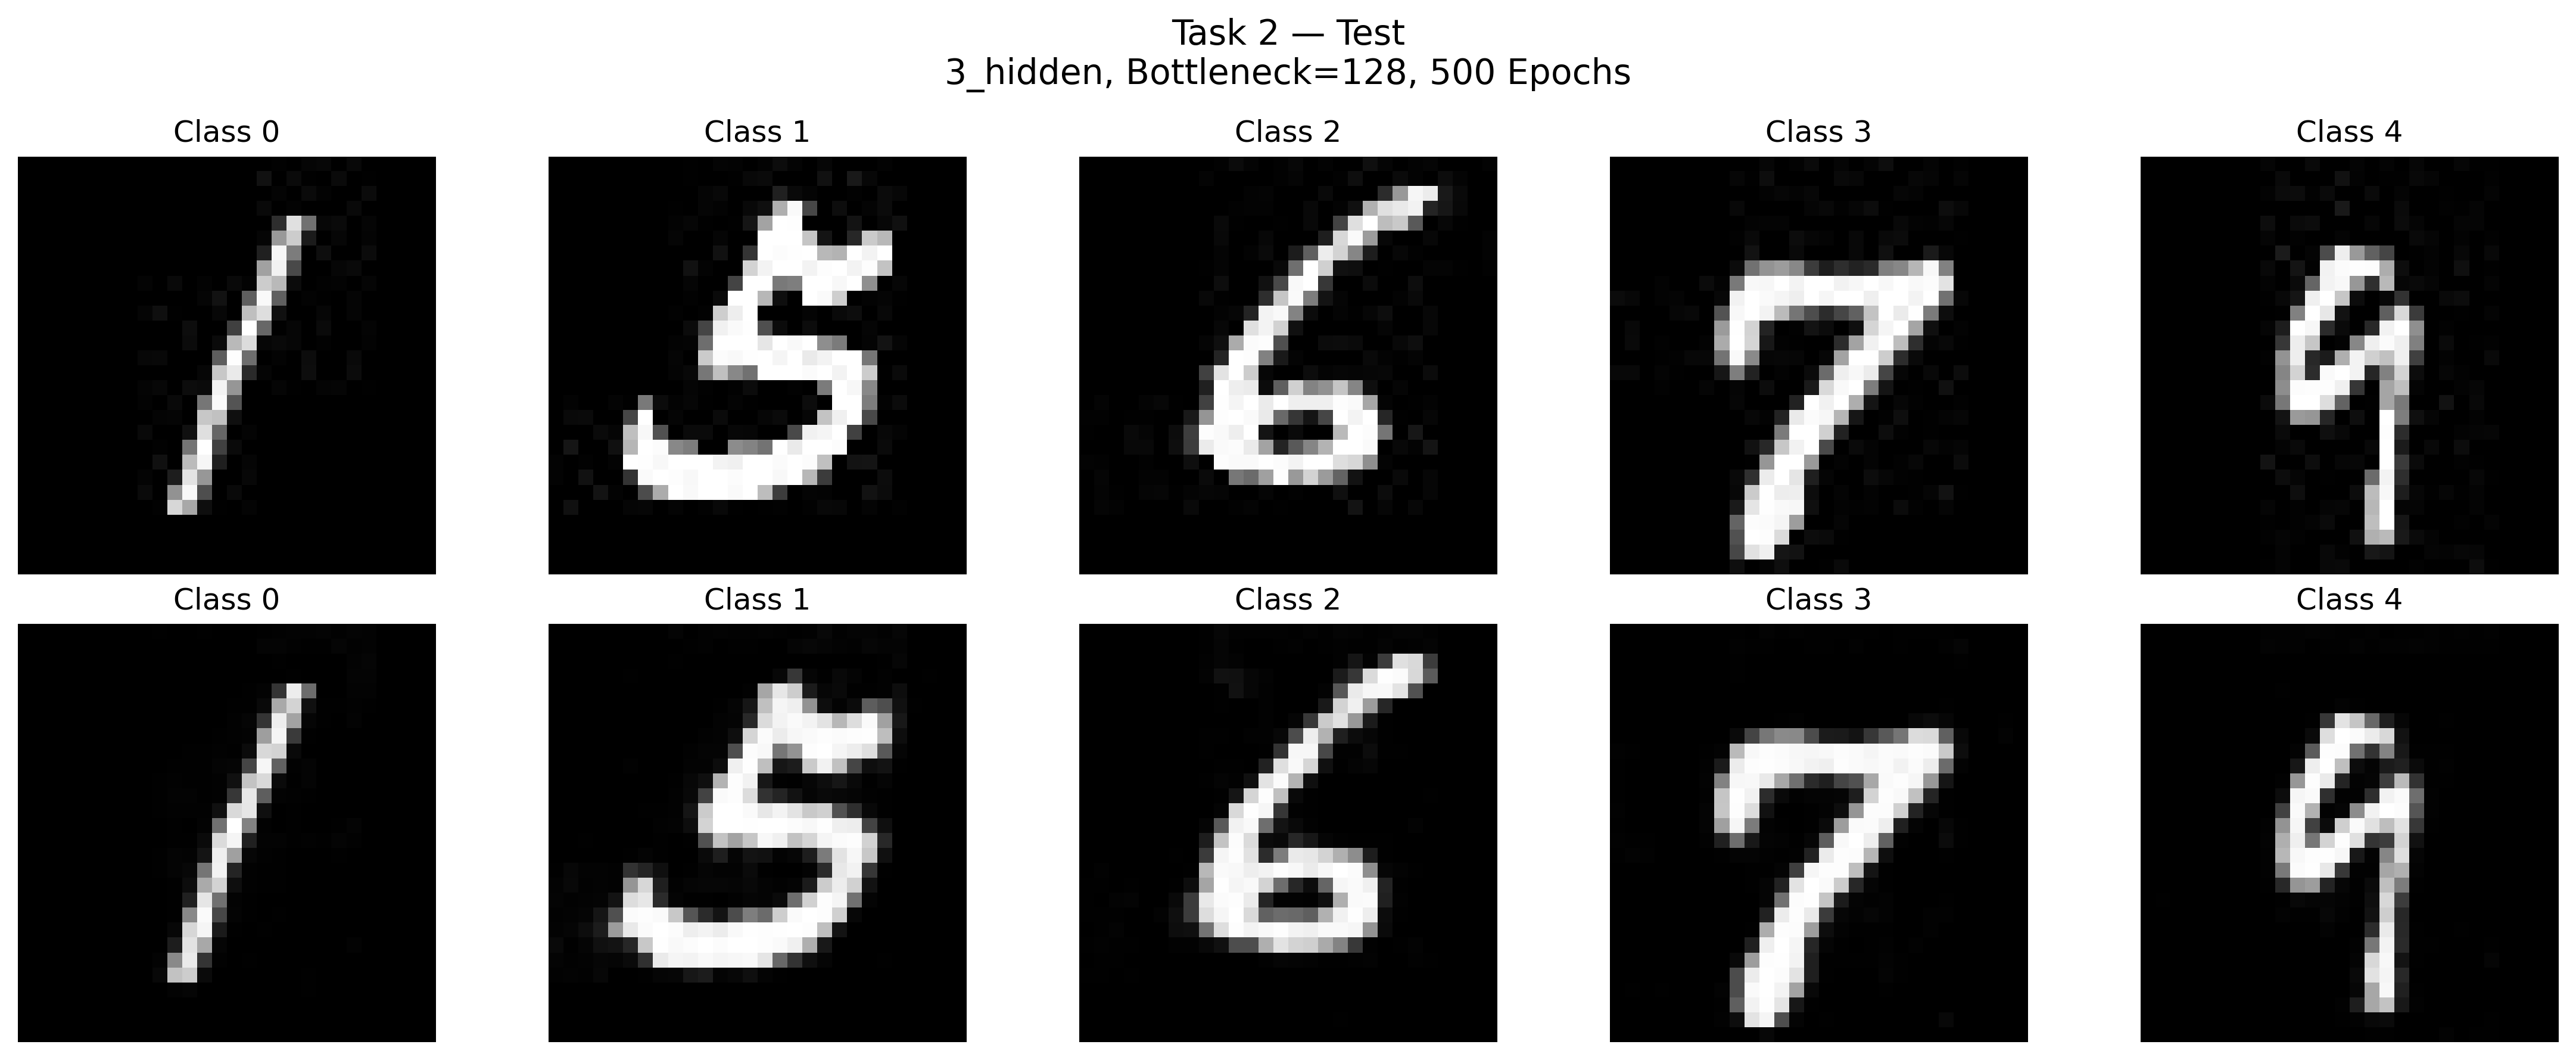
\includegraphics[width=0.96\linewidth,height=0.48\textheight,keepaspectratio]{figures/task2/model_reconstruction_visualization_500/test_3_hidden_bottleneck_128_500epochs.png}
\caption{Autoencoder reconstruction visualization: test 3 hidden with bottleneck of 128 neurons.}
\label{fig:task2_7}
\end{figure}

\begin{figure}[H]
\centering
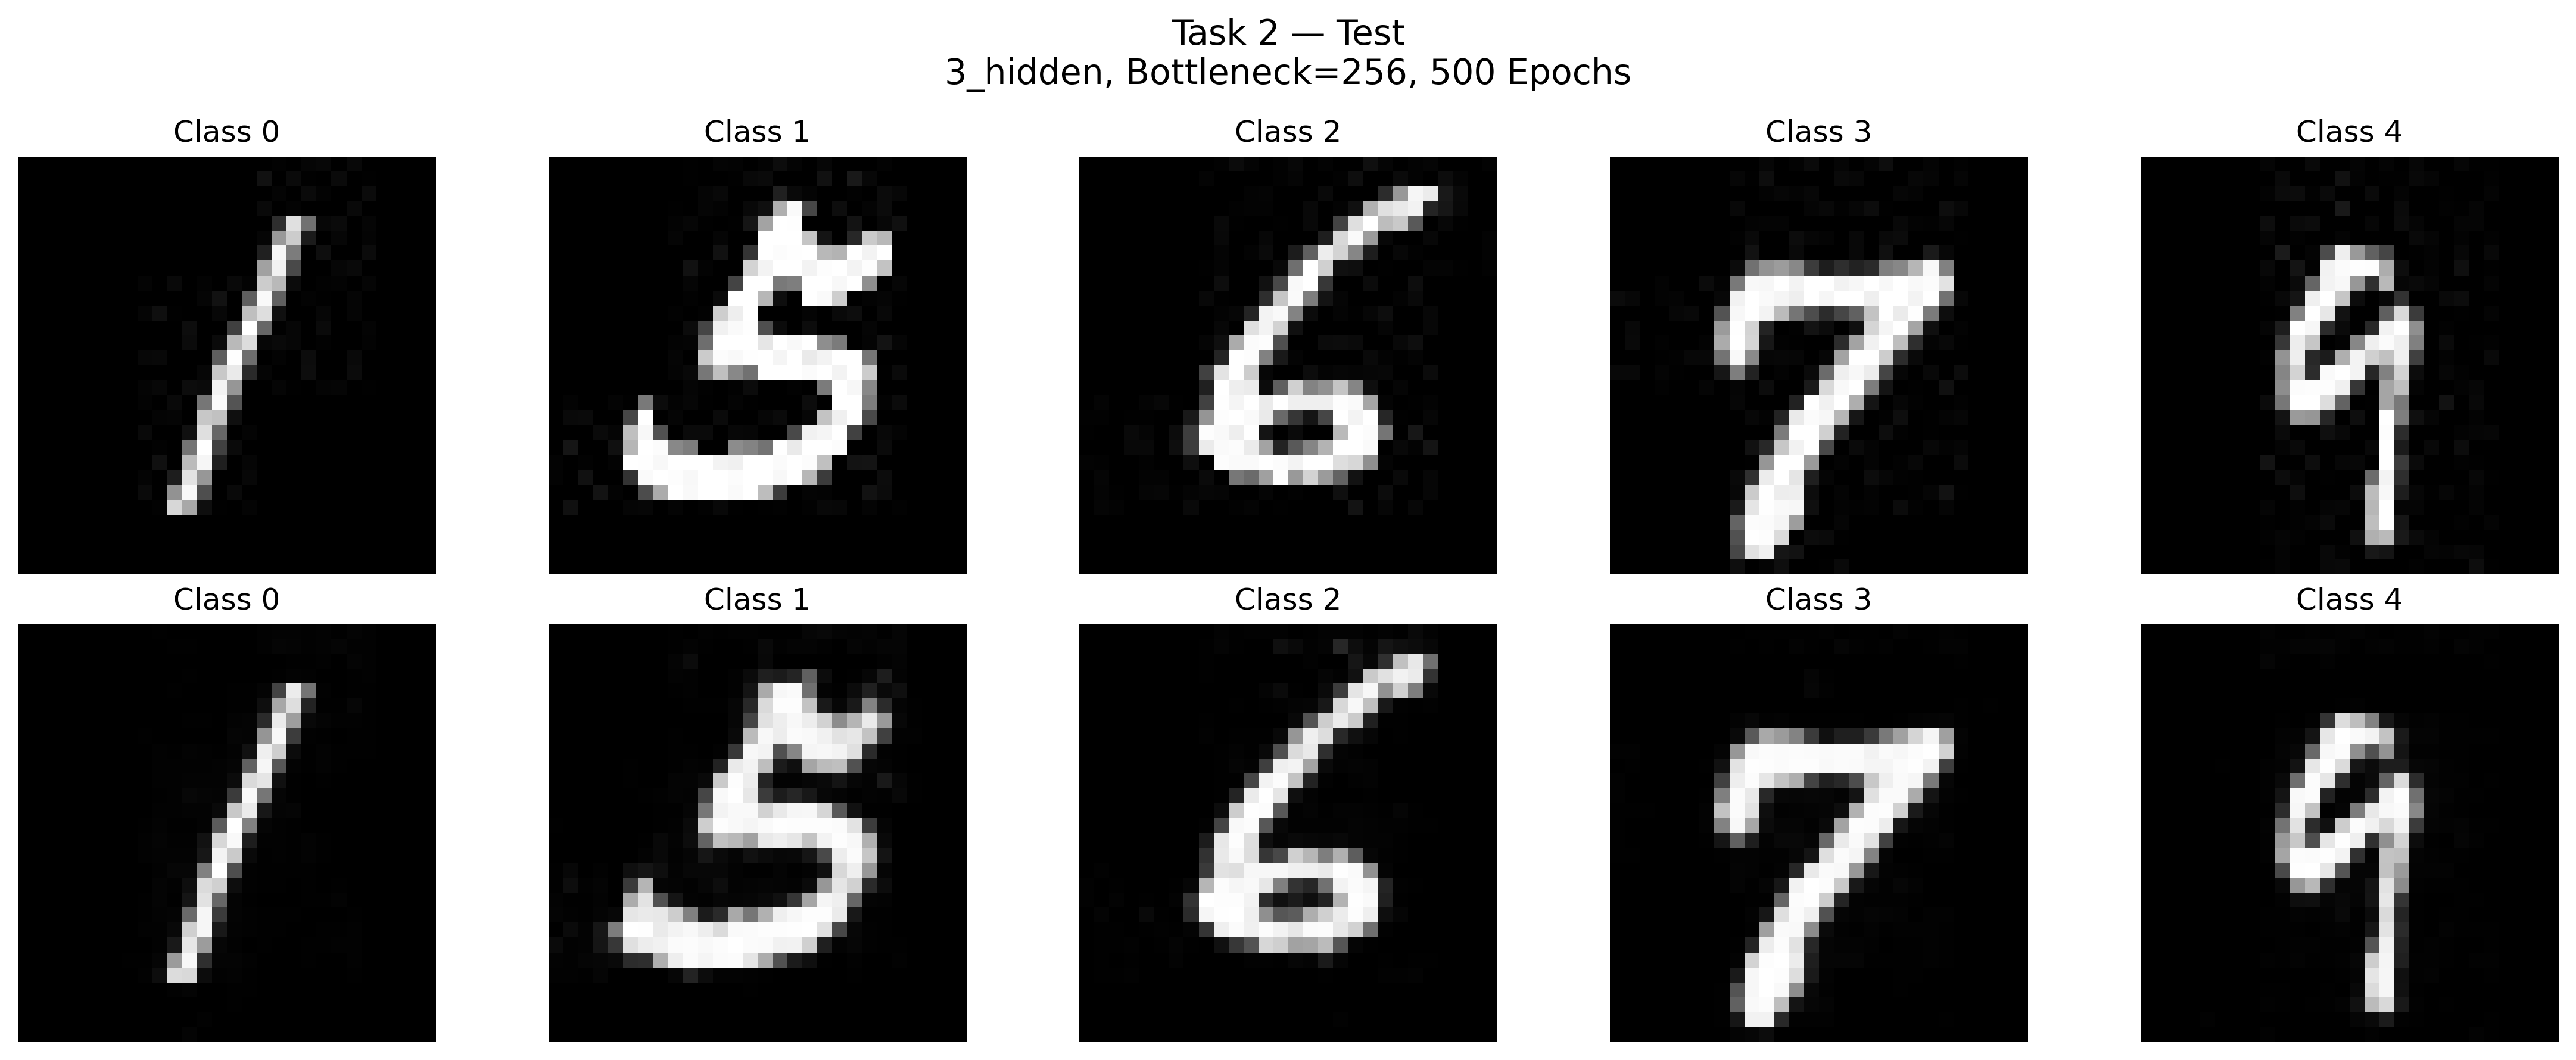
\includegraphics[width=0.96\linewidth,height=0.48\textheight,keepaspectratio]{figures/task2/model_reconstruction_visualization_500/test_3_hidden_bottleneck_256_500epochs.png}
\caption{Autoencoder reconstruction visualization: test 3 hidden with bottleneck of 256 neurons.}
\label{fig:task2_8}
\end{figure}

\begin{figure}[H]
\centering
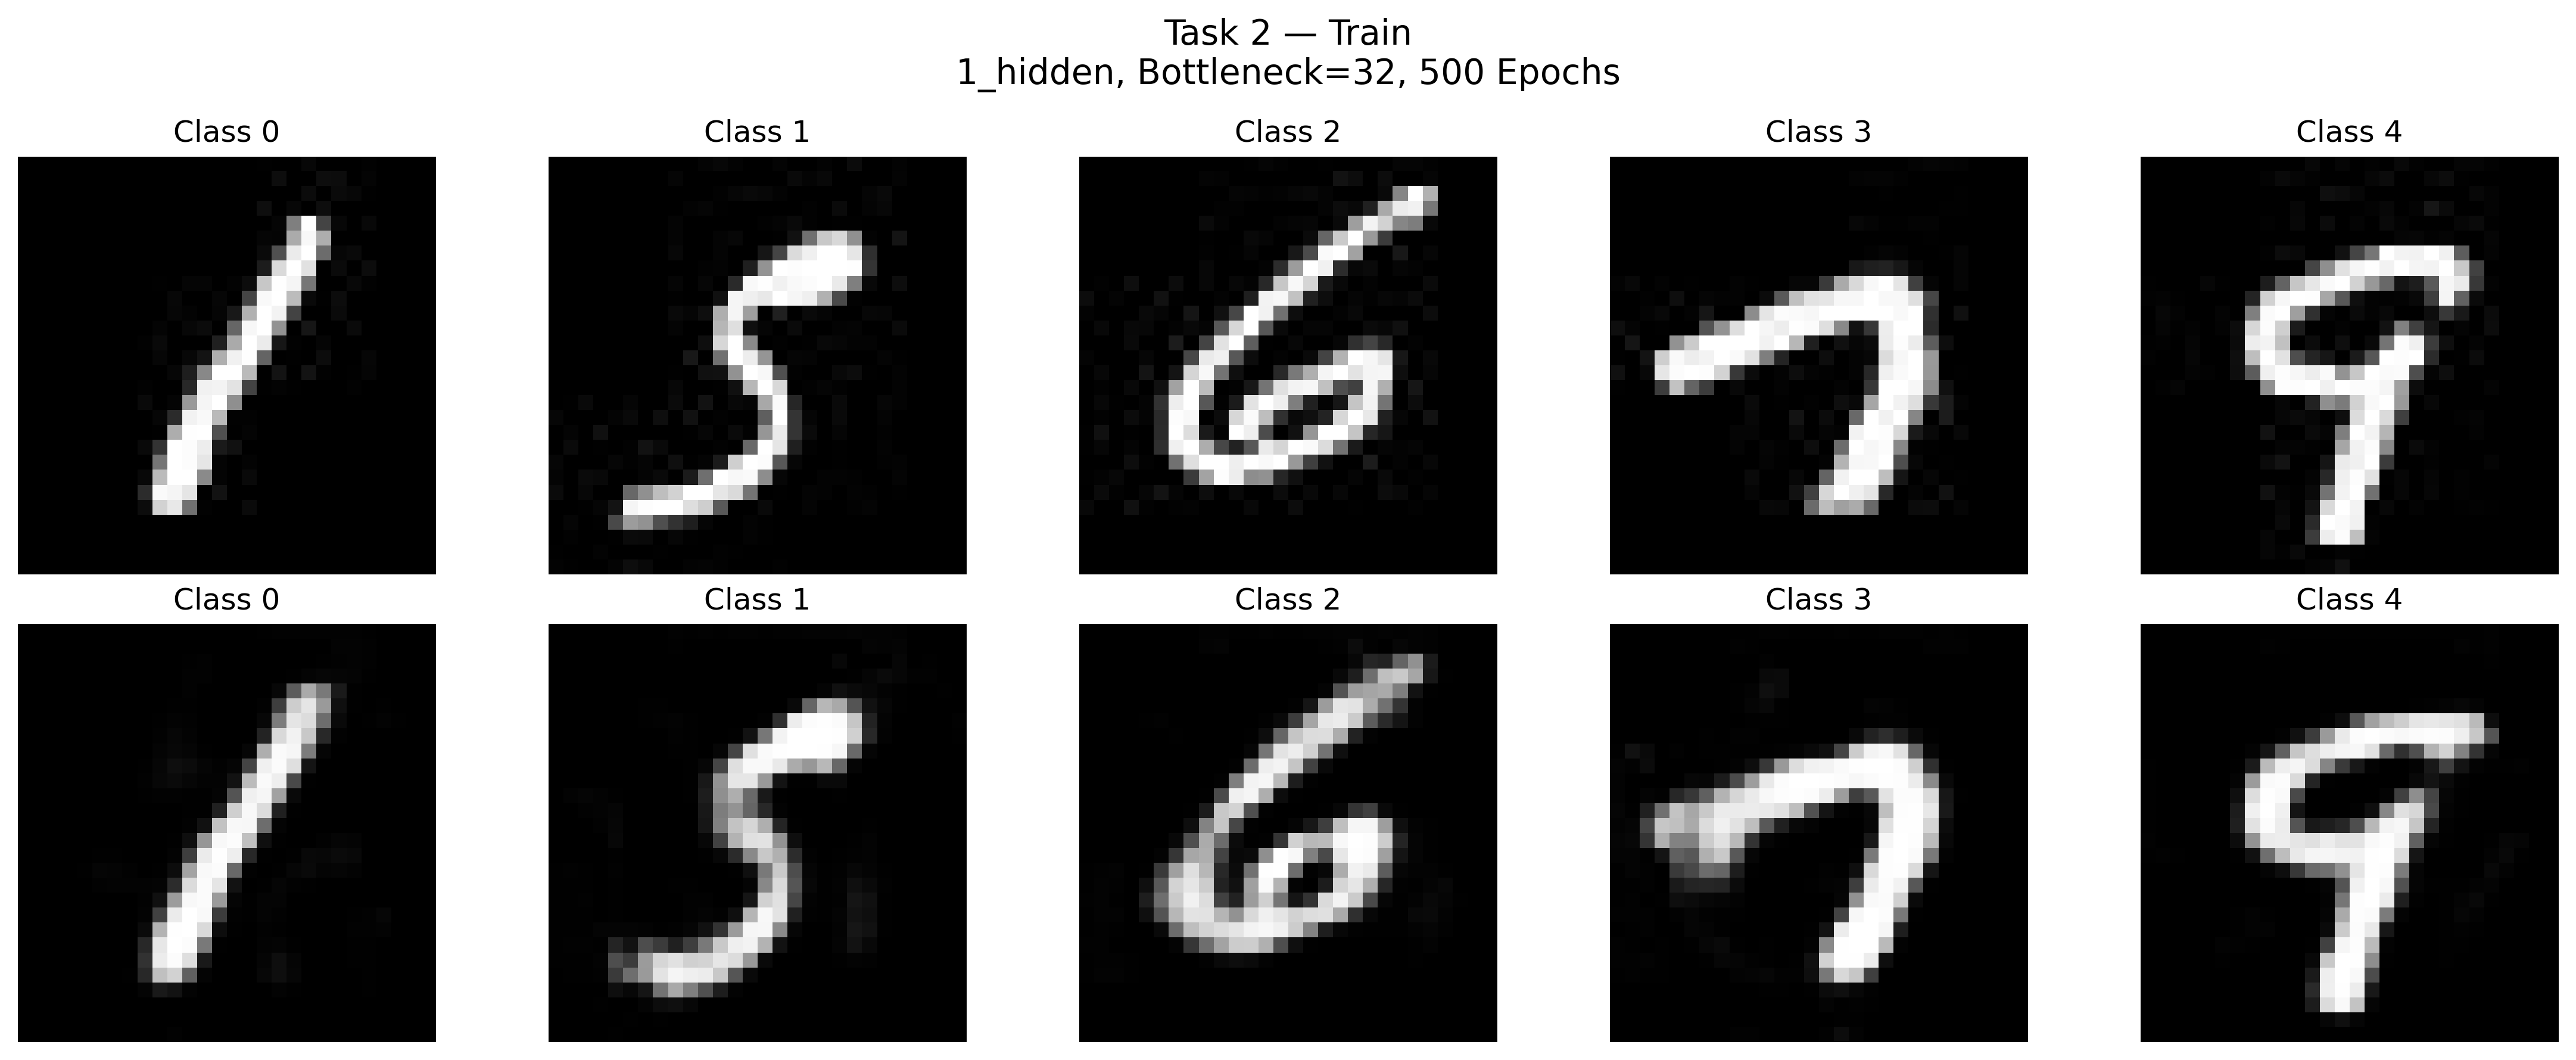
\includegraphics[width=0.96\linewidth,height=0.48\textheight,keepaspectratio]{figures/task2/model_reconstruction_visualization_500/train_1_hidden_bottleneck_32_500epochs.png}
\caption{Autoencoder reconstruction visualization: train 1 hidden with bottleneck of 32 neurons.}
\label{fig:task2_9}
\end{figure}

\begin{figure}[H]
\centering
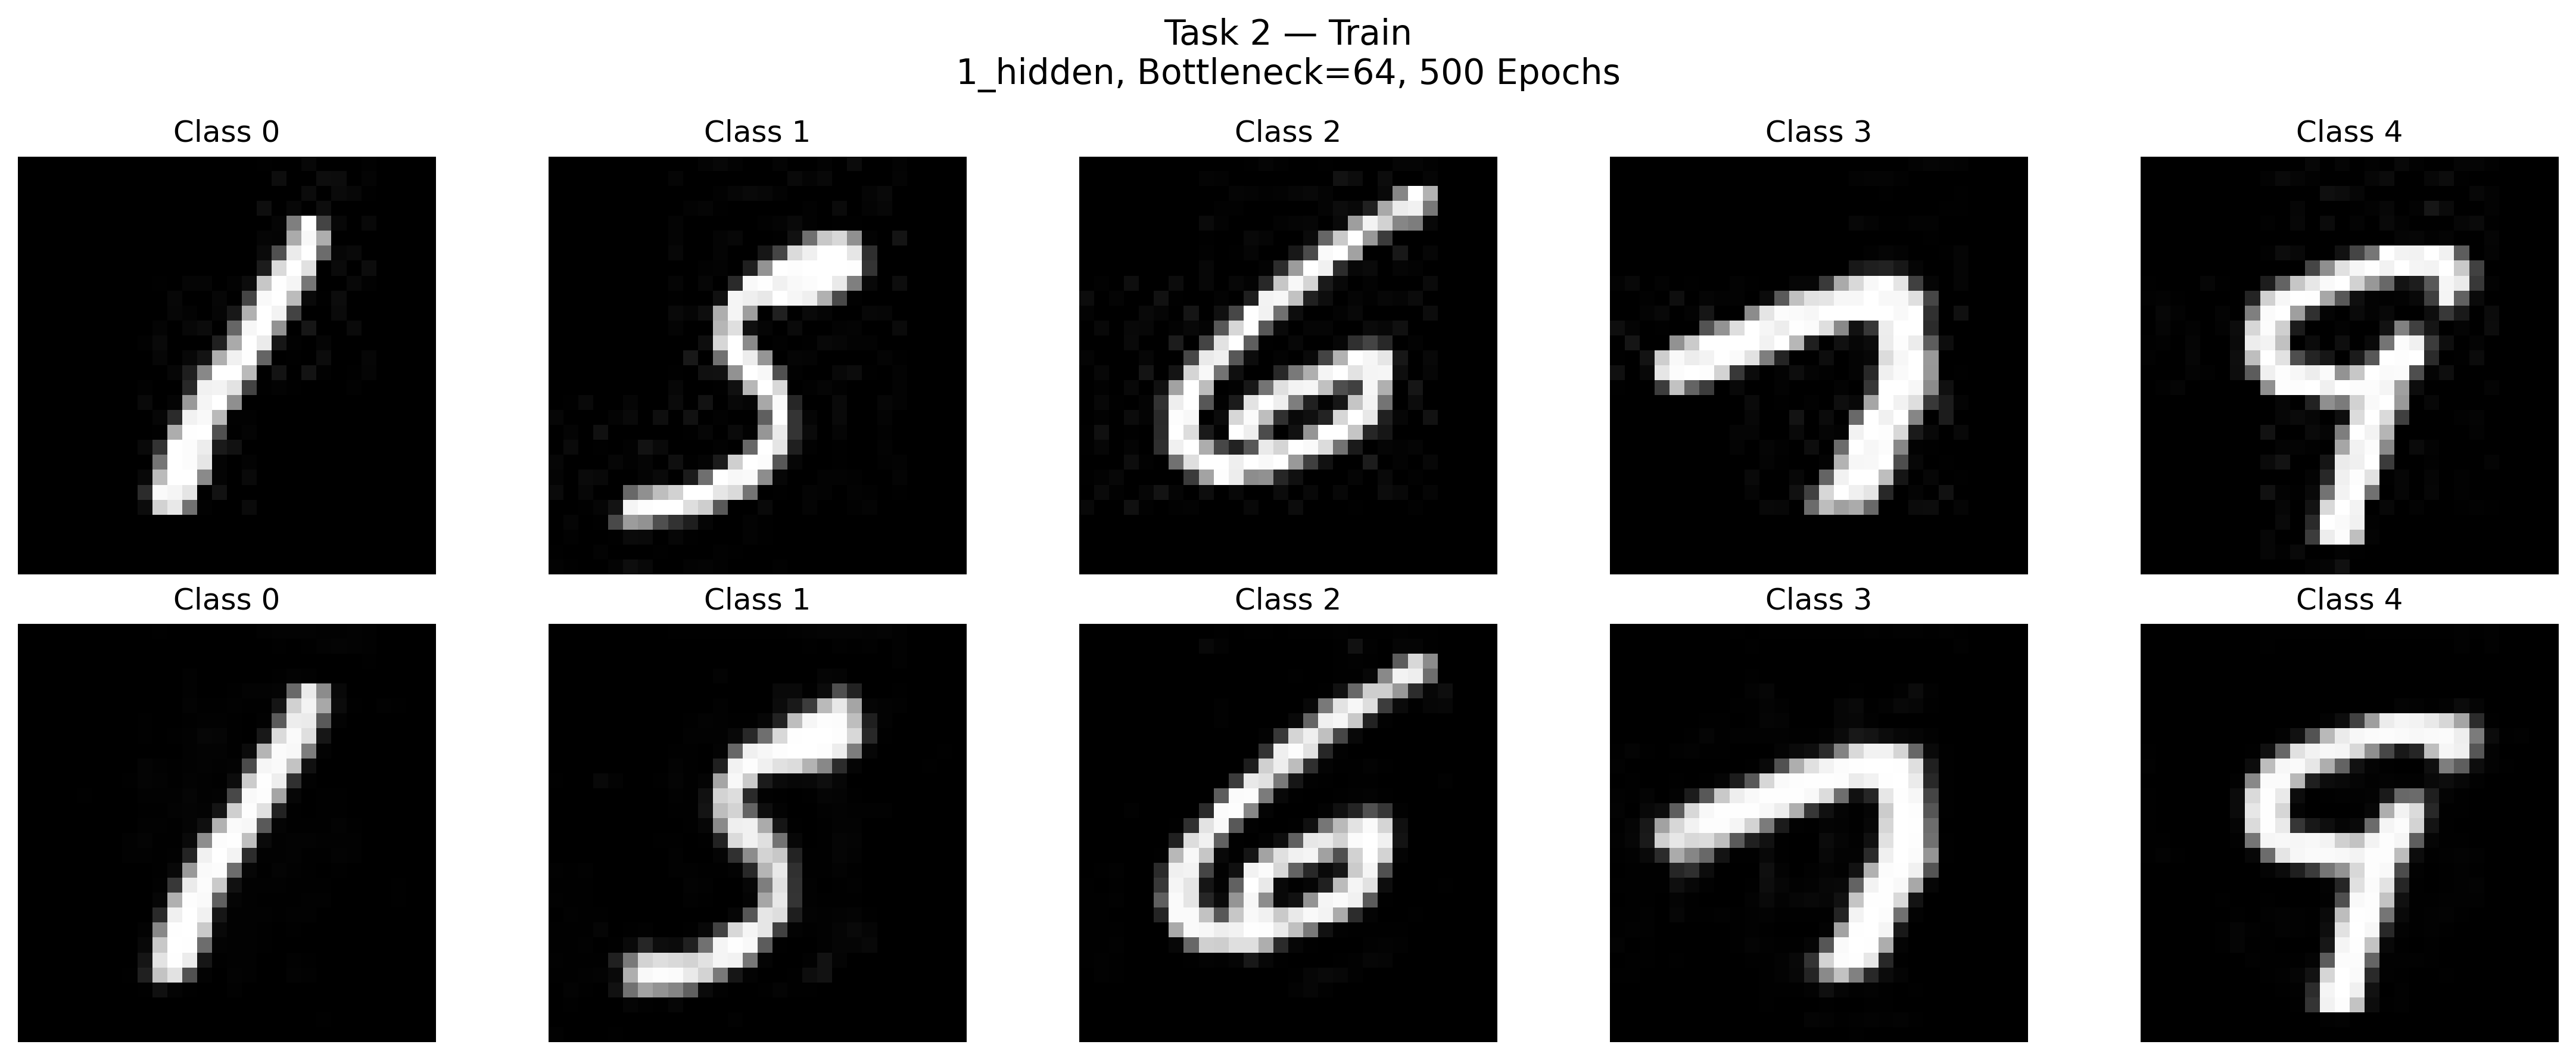
\includegraphics[width=0.96\linewidth,height=0.48\textheight,keepaspectratio]{figures/task2/model_reconstruction_visualization_500/train_1_hidden_bottleneck_64_500epochs.png}
\caption{Autoencoder reconstruction visualization: train 1 hidden with bottleneck of 64 neurons.}
\label{fig:task2_10}
\end{figure}

\begin{figure}[H]
\centering
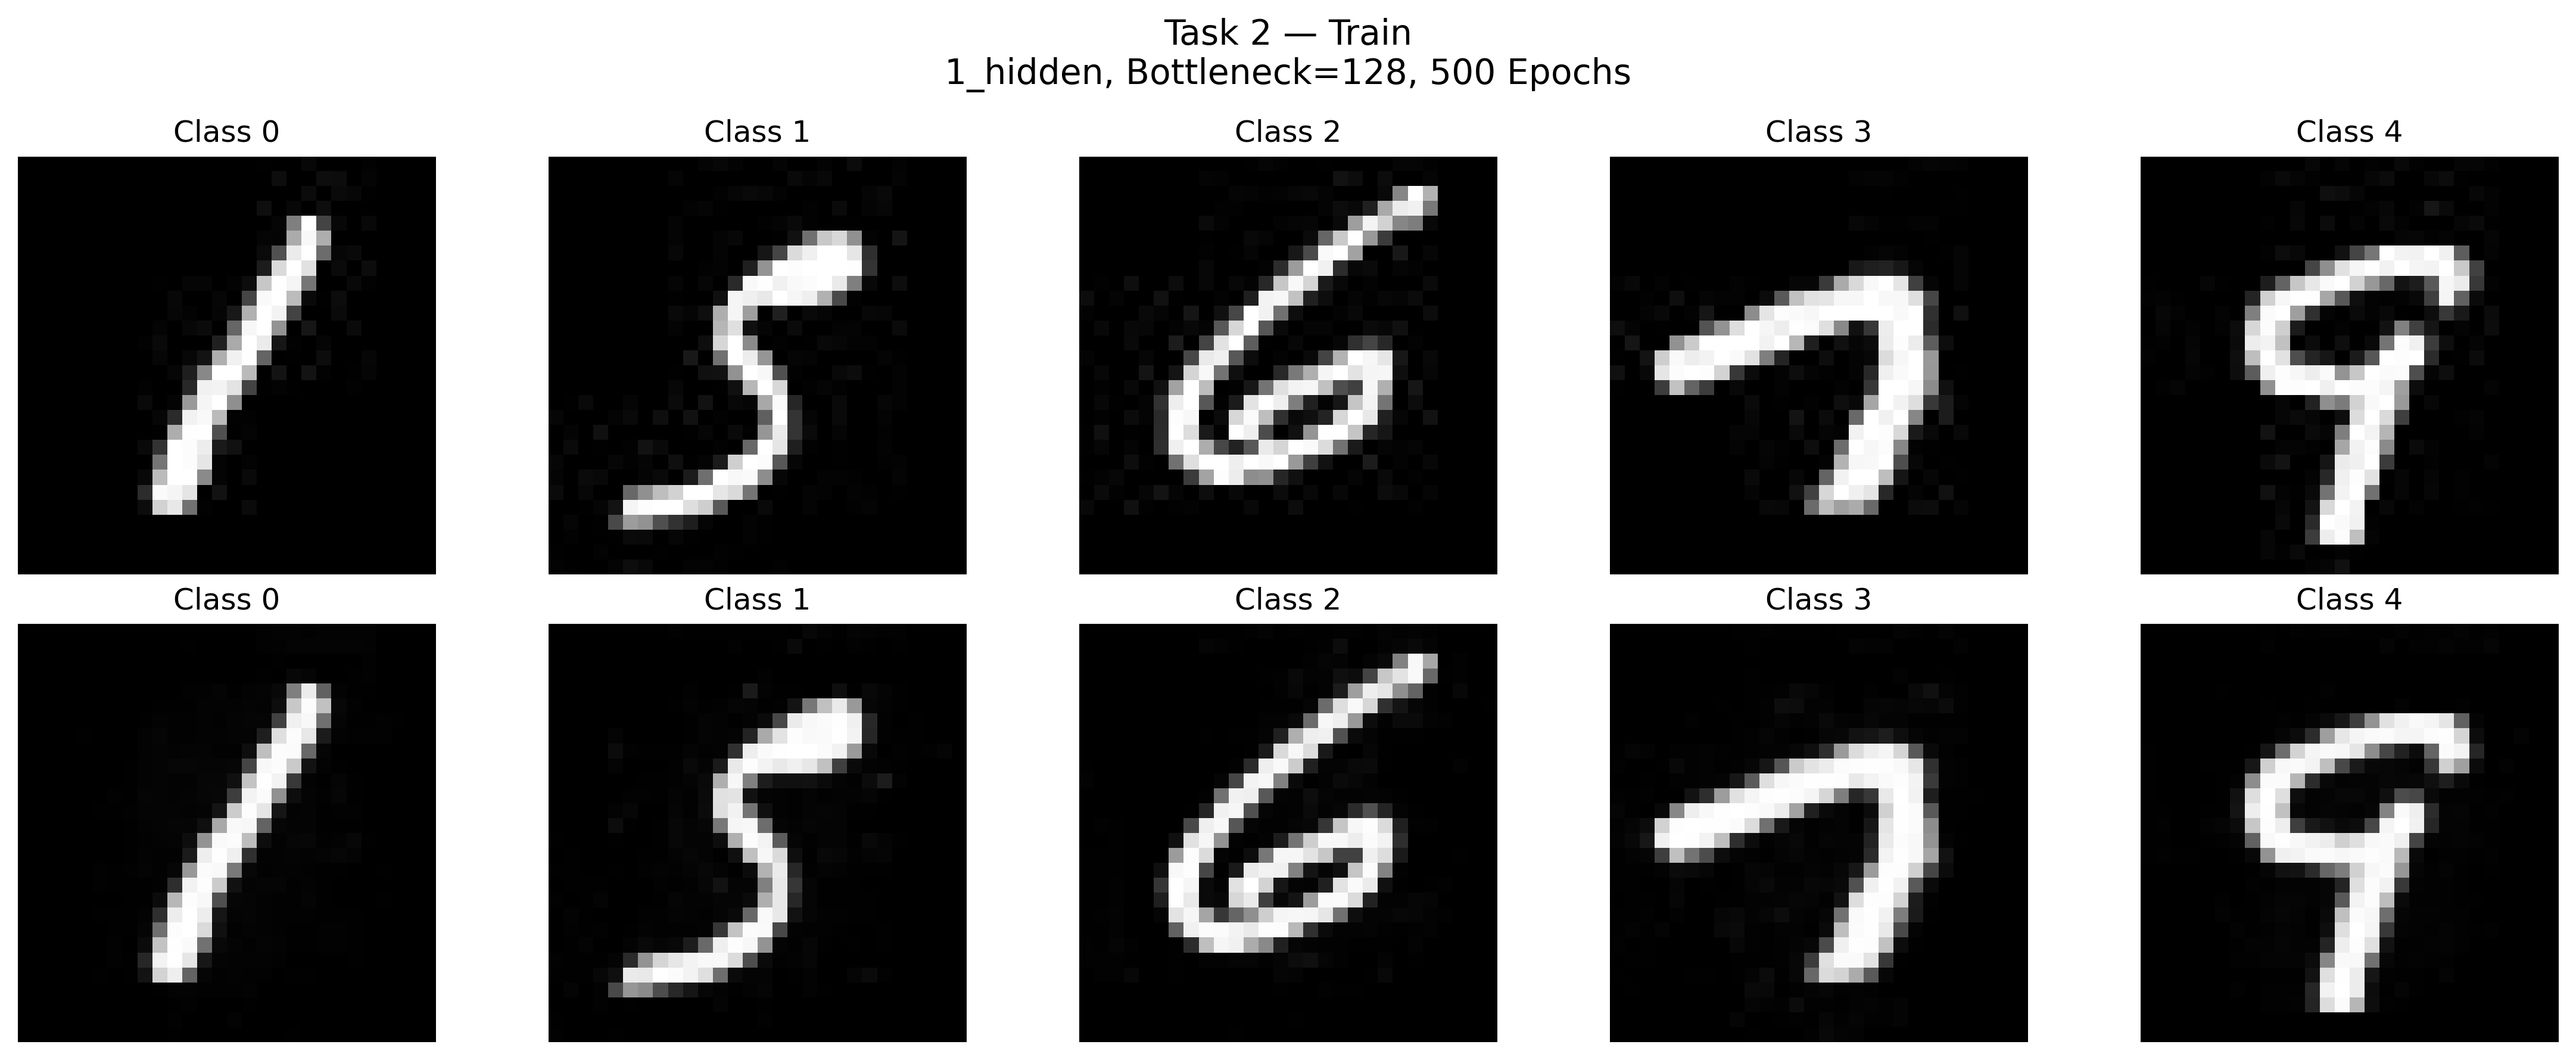
\includegraphics[width=0.96\linewidth,height=0.48\textheight,keepaspectratio]{figures/task2/model_reconstruction_visualization_500/train_1_hidden_bottleneck_128_500epochs.png}
\caption{Autoencoder reconstruction visualization: train 1 hidden with bottleneck of 128 neurons.}
\label{fig:task2_11}
\end{figure}

\begin{figure}[H]
\centering
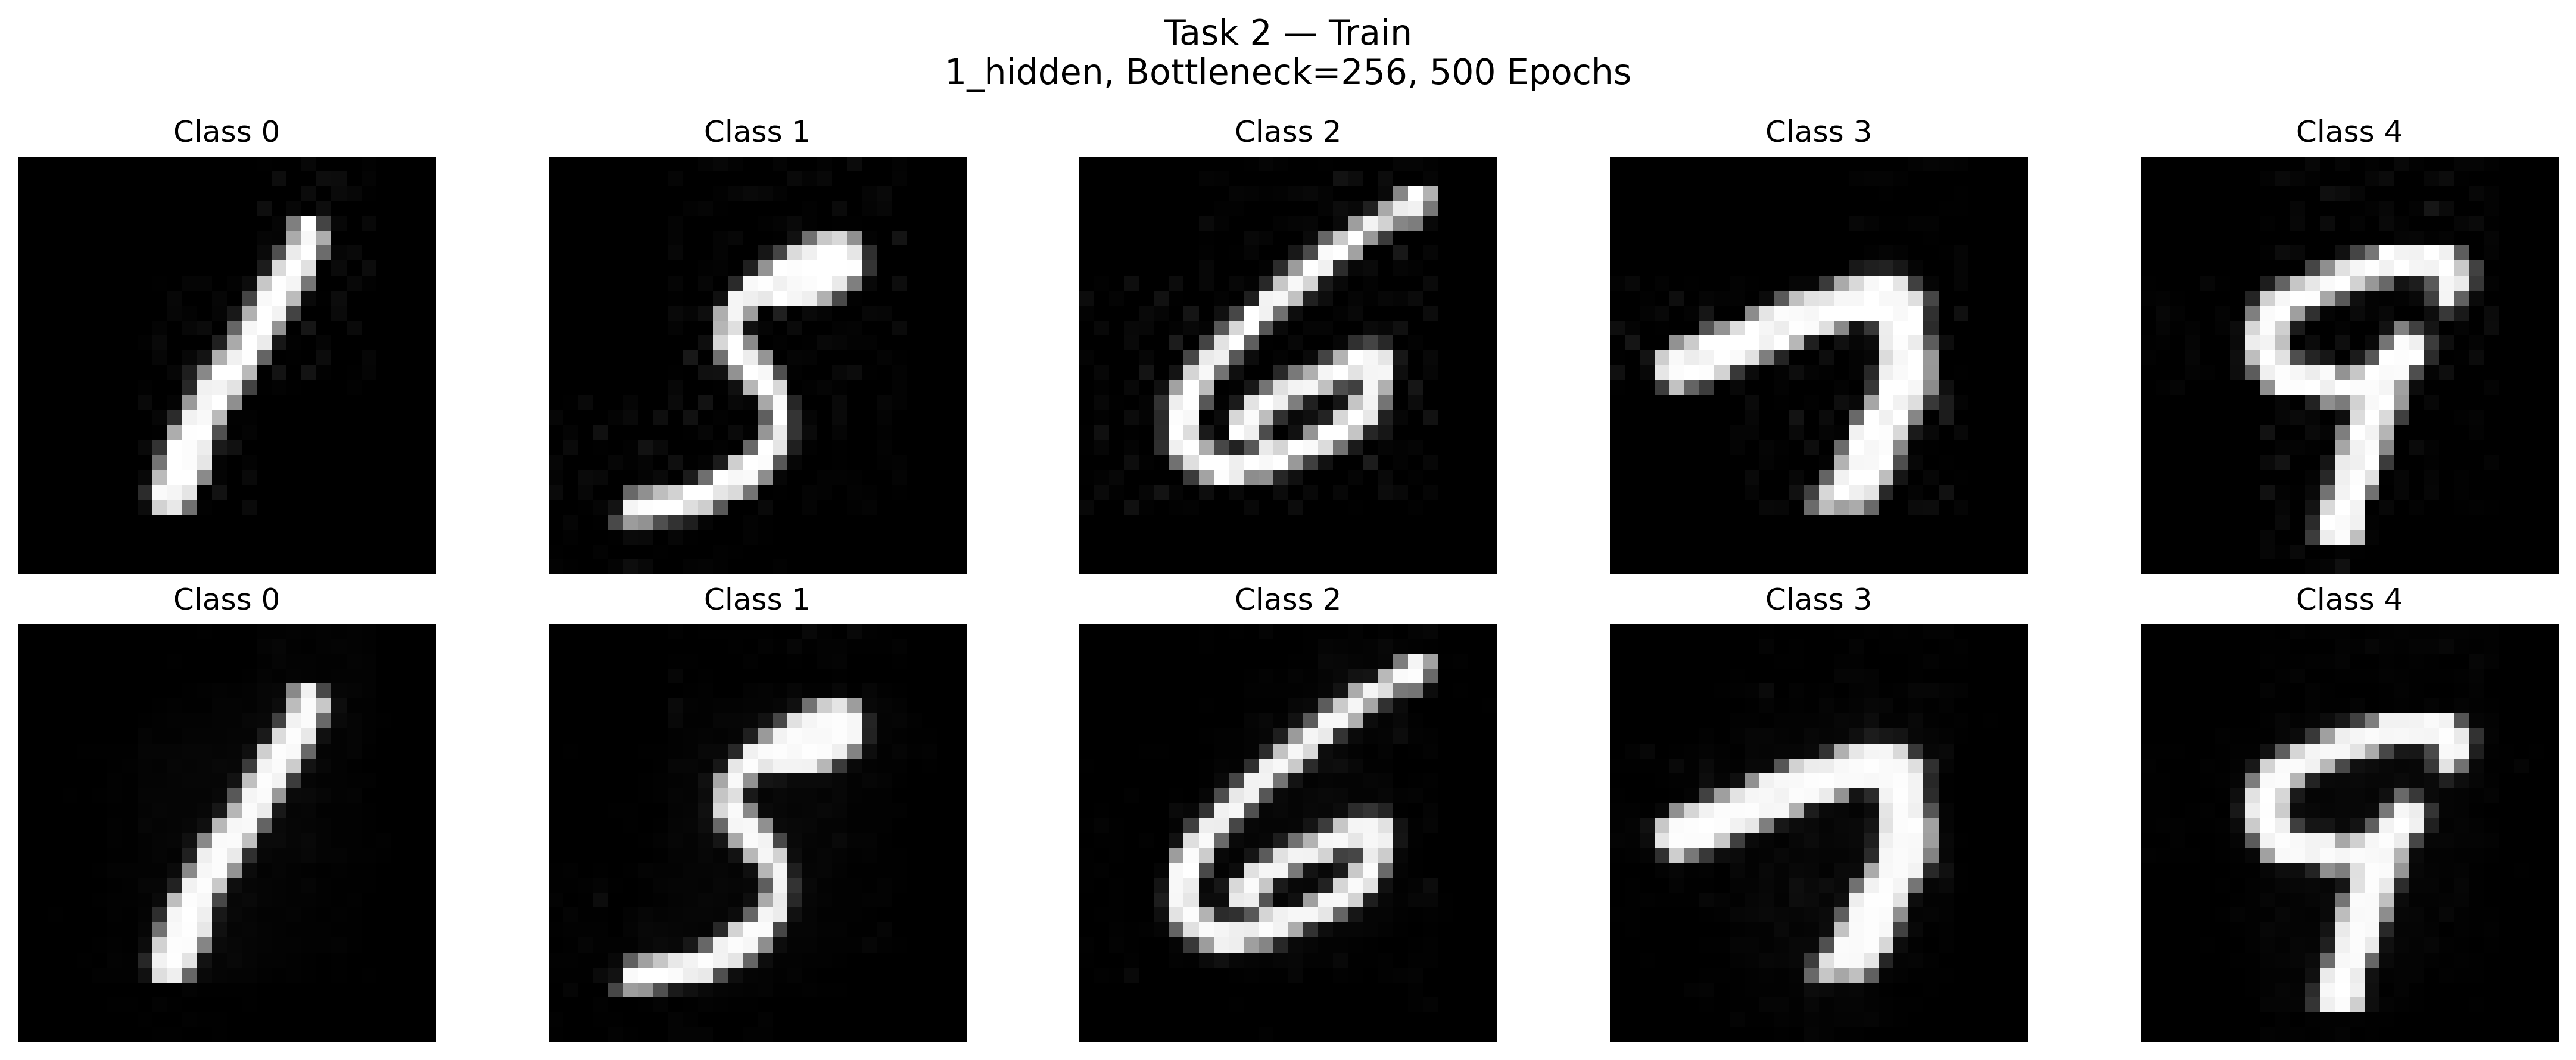
\includegraphics[width=0.96\linewidth,height=0.48\textheight,keepaspectratio]{figures/task2/model_reconstruction_visualization_500/train_1_hidden_bottleneck_256_500epochs.png}
\caption{Autoencoder reconstruction visualization: train 1 hidden with bottleneck of 256 neurons.}
\label{fig:task2_12}
\end{figure}

\begin{figure}[H]
\centering
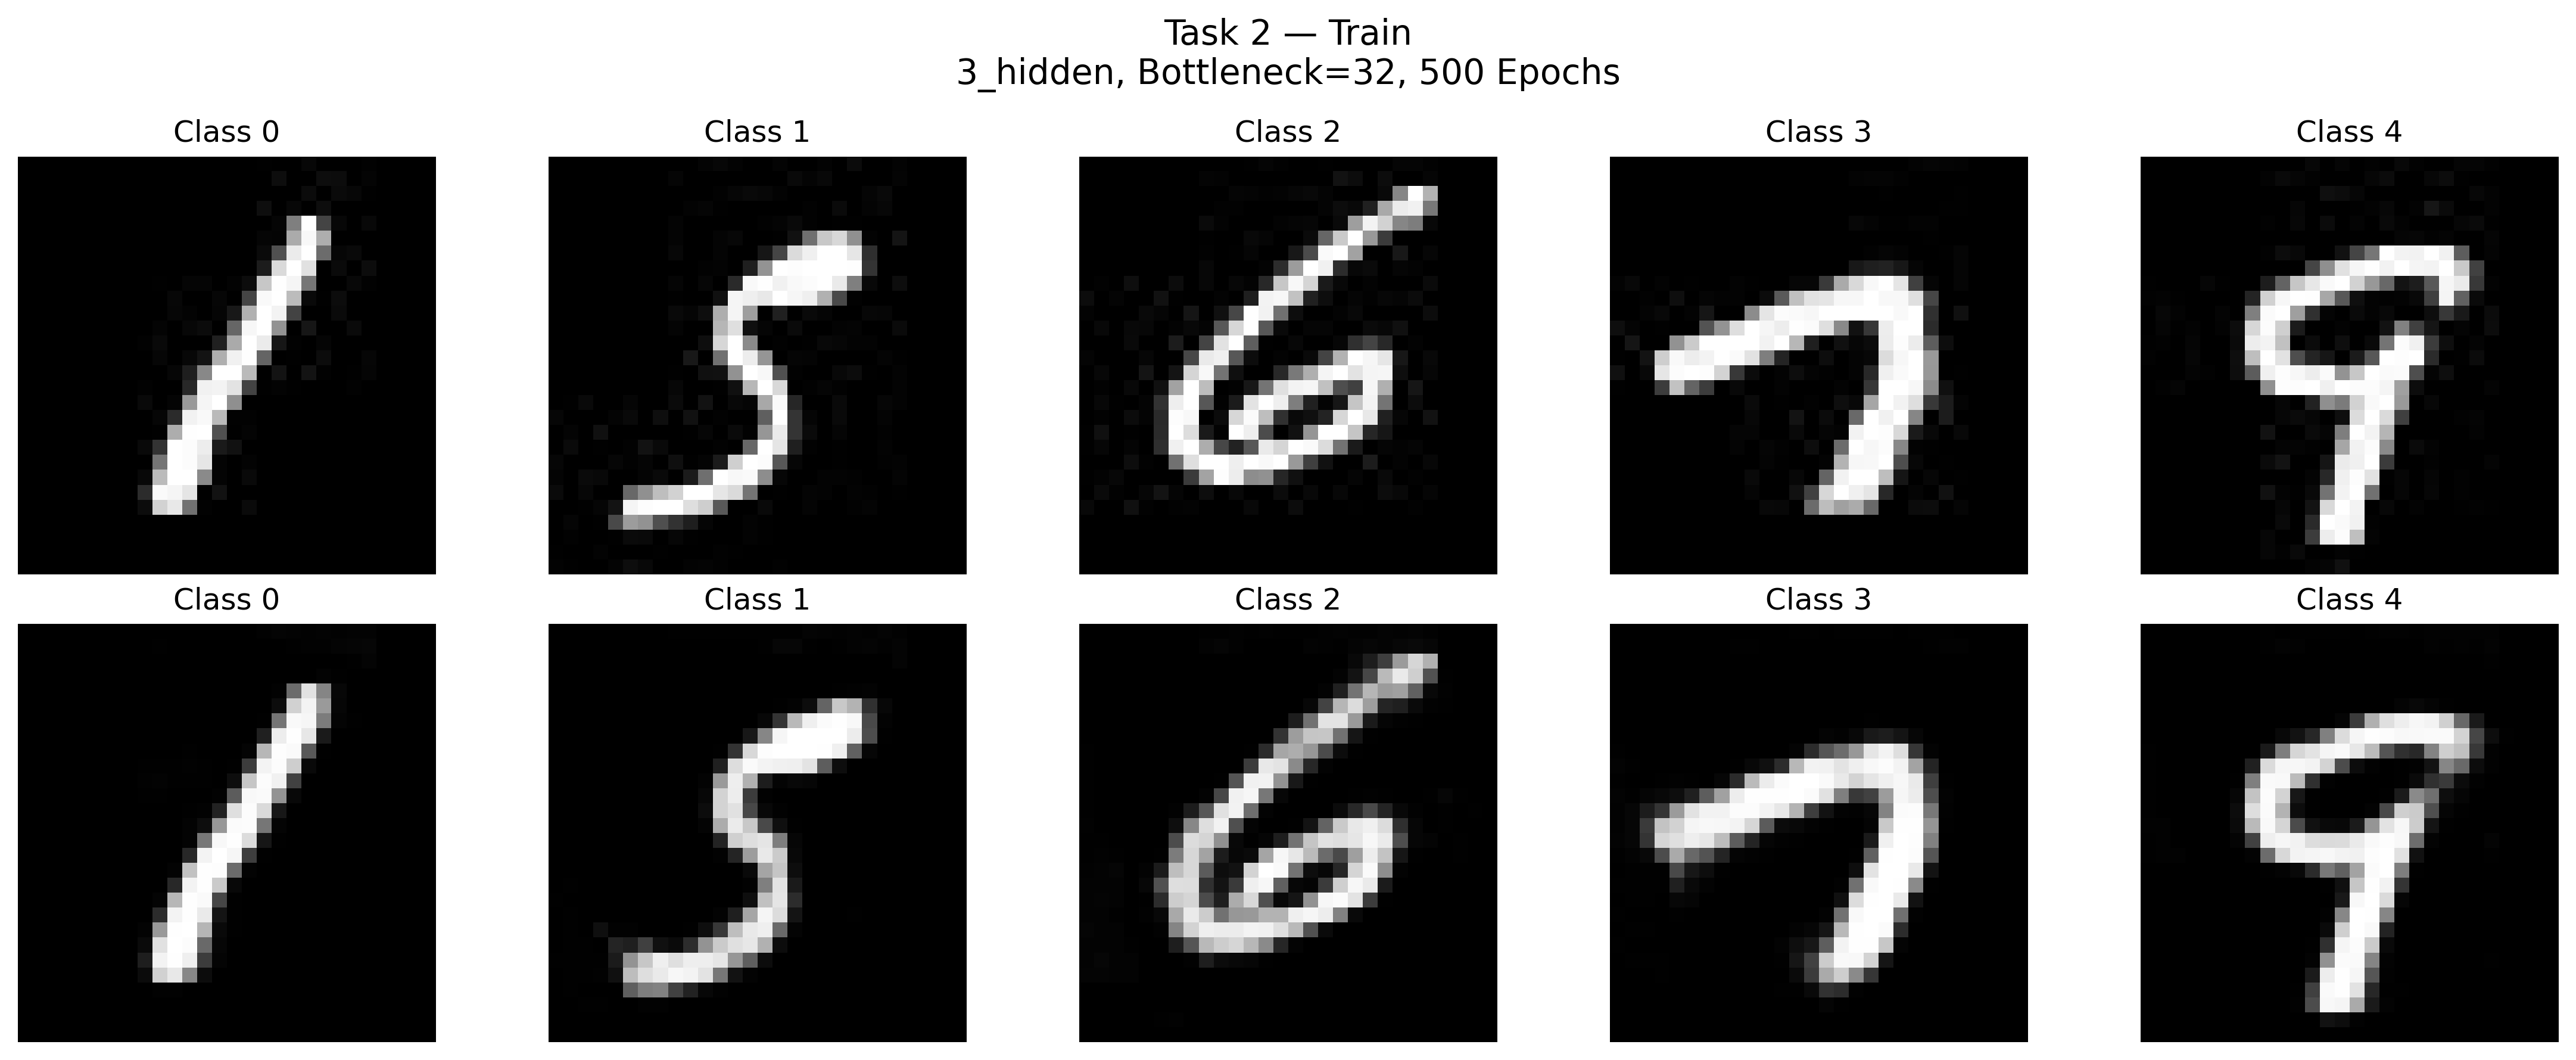
\includegraphics[width=0.96\linewidth,height=0.48\textheight,keepaspectratio]{figures/task2/model_reconstruction_visualization_500/train_3_hidden_bottleneck_32_500epochs.png}
\caption{Autoencoder reconstruction visualization: train 3 hidden with bottleneck of 32 neurons.}
\label{fig:task2_13}
\end{figure}

\begin{figure}[H]
\centering
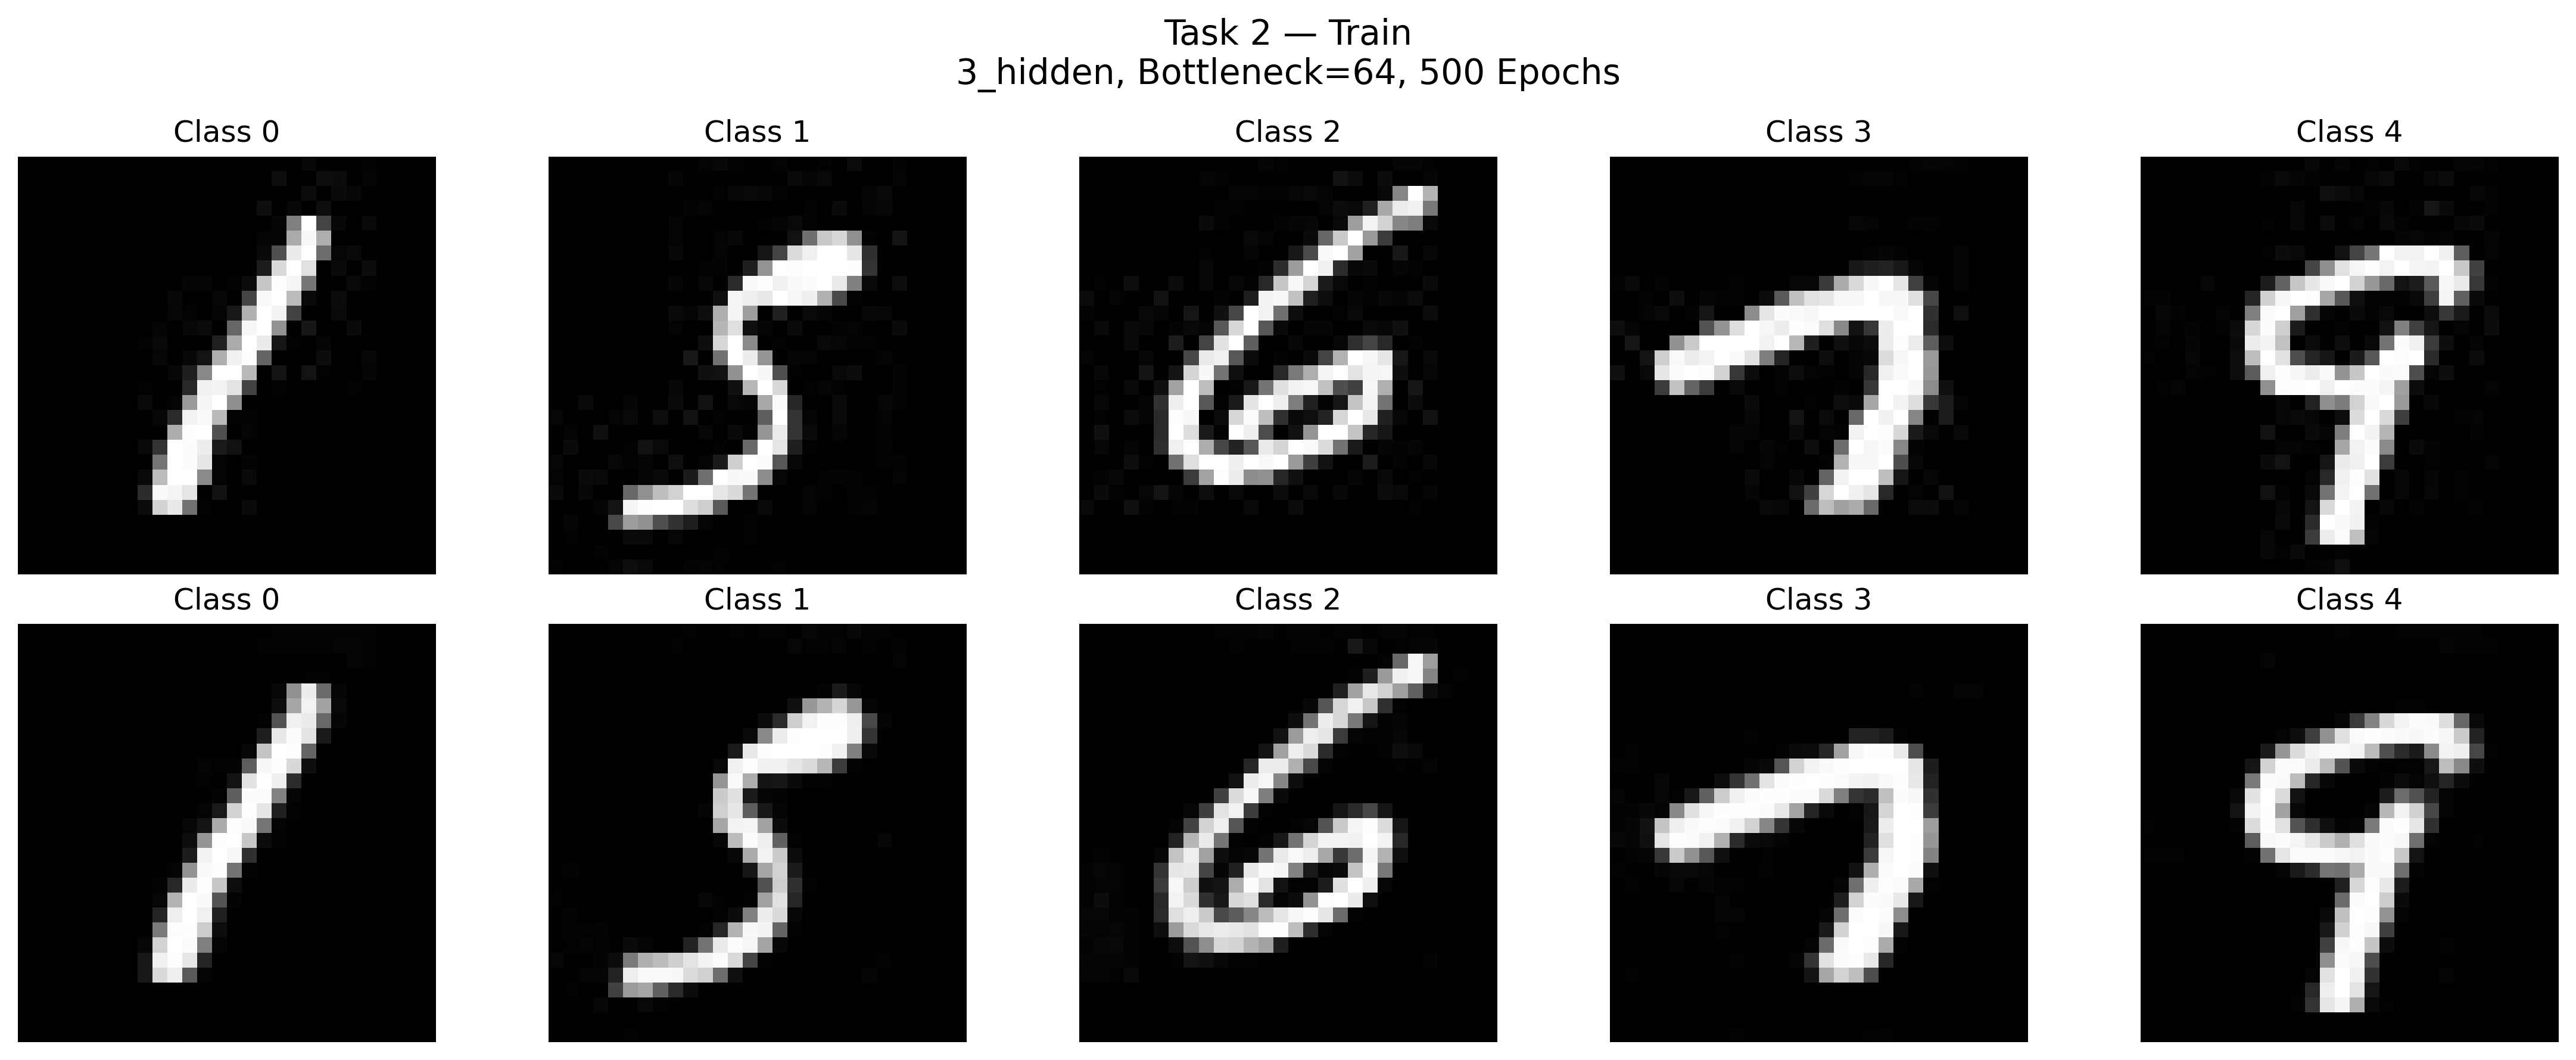
\includegraphics[width=0.96\linewidth,height=0.48\textheight,keepaspectratio]{figures/task2/model_reconstruction_visualization_500/train_3_hidden_bottleneck_64_500epochs.png}
\caption{Autoencoder reconstruction visualization: train 3 hidden with bottleneck of 64 neurons.}
\label{fig:task2_14}
\end{figure}

\begin{figure}[H]
\centering
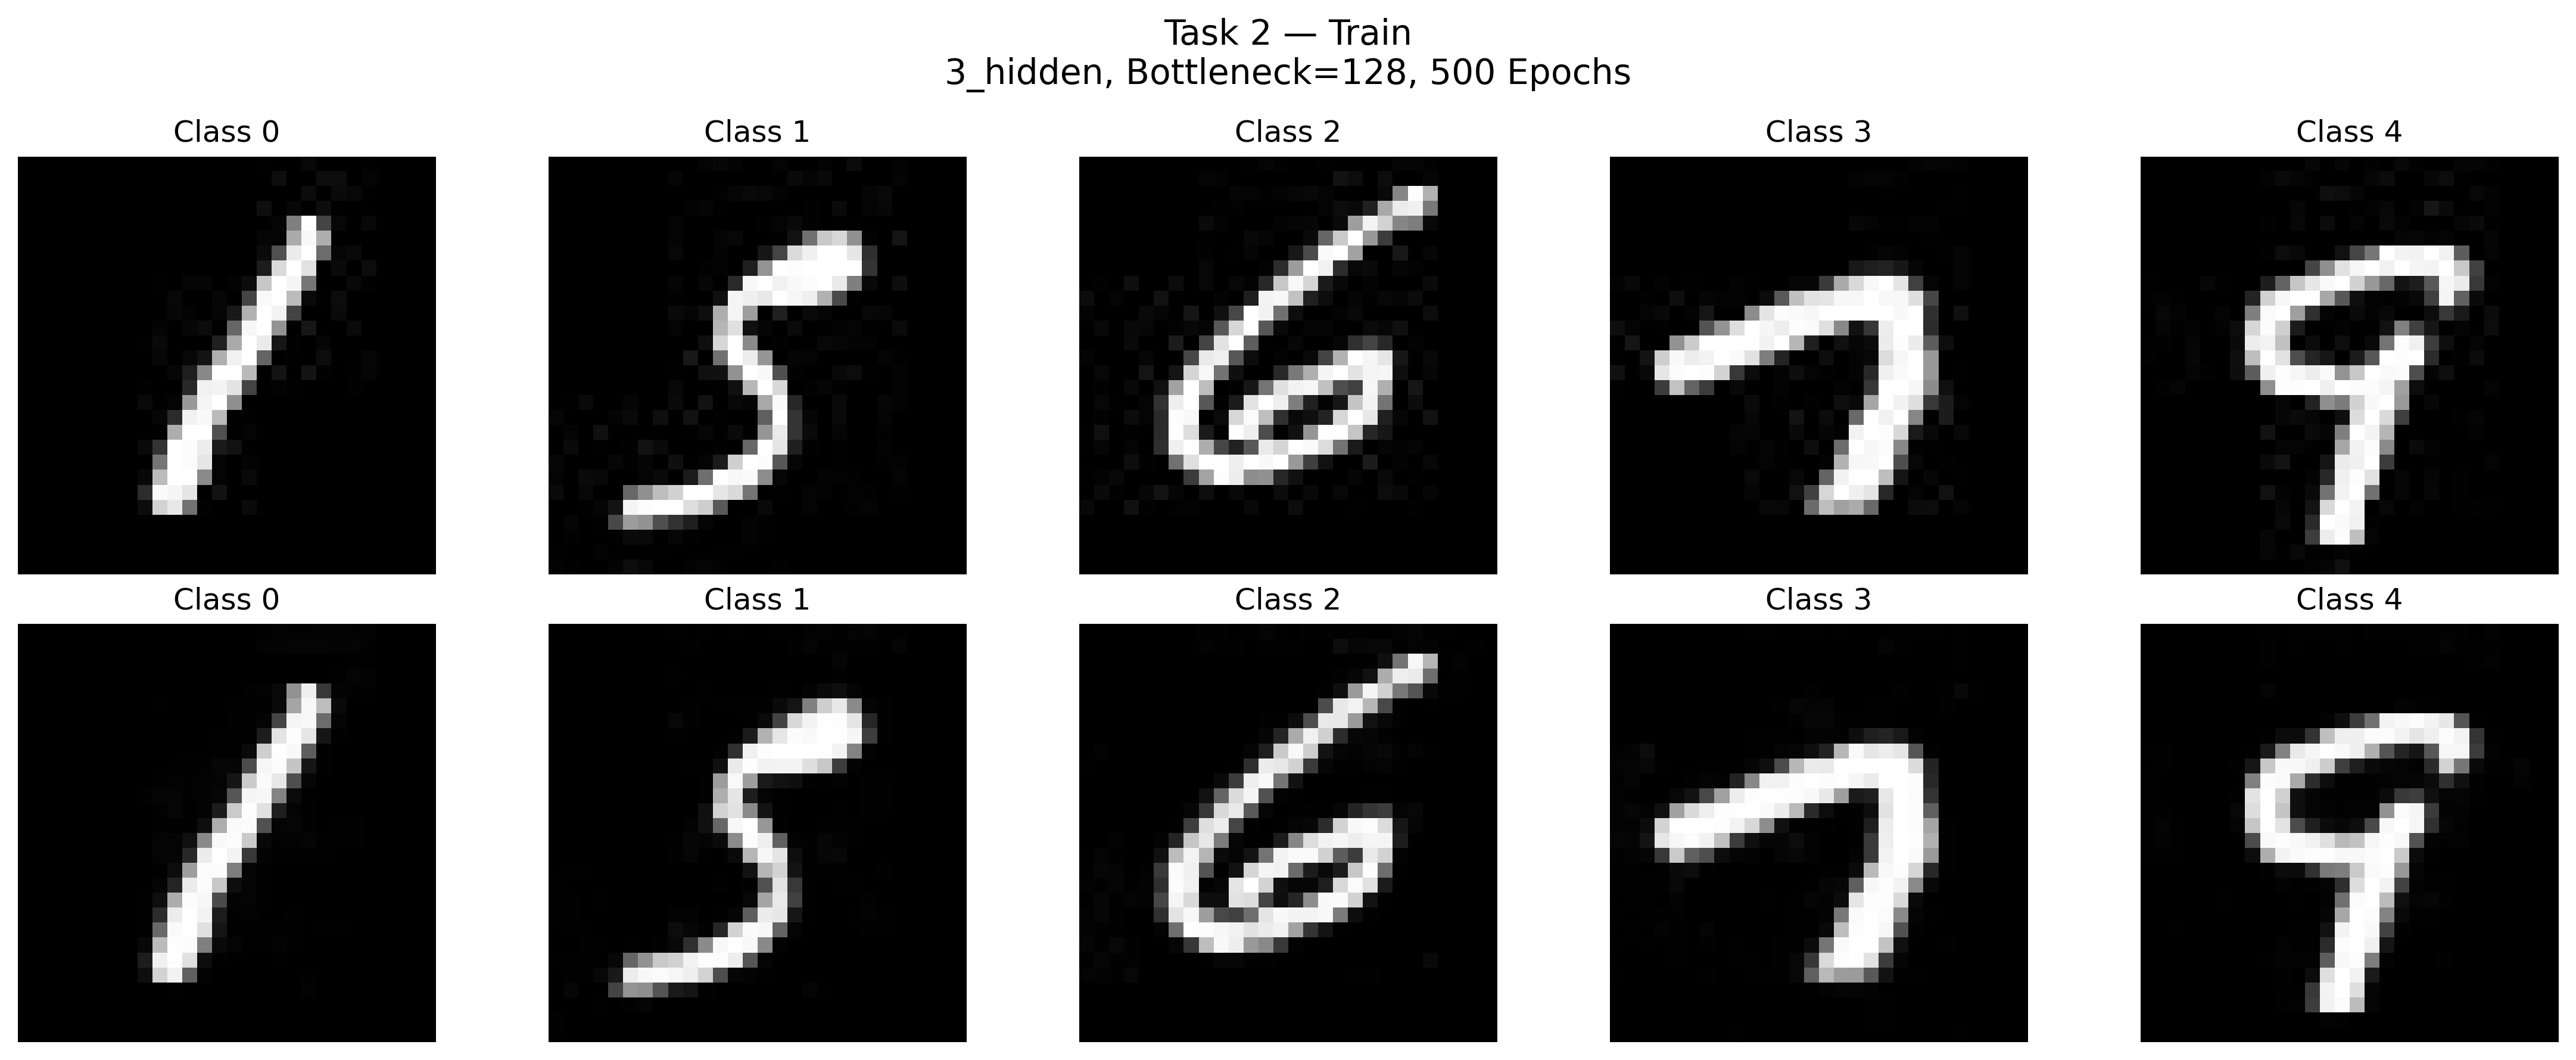
\includegraphics[width=0.96\linewidth,height=0.48\textheight,keepaspectratio]{figures/task2/model_reconstruction_visualization_500/train_3_hidden_bottleneck_128_500epochs.png}
\caption{Autoencoder reconstruction visualization: train 3 hidden with bottleneck of 128 neurons.}
\label{fig:task2_15}
\end{figure}

\begin{figure}[H]
\centering
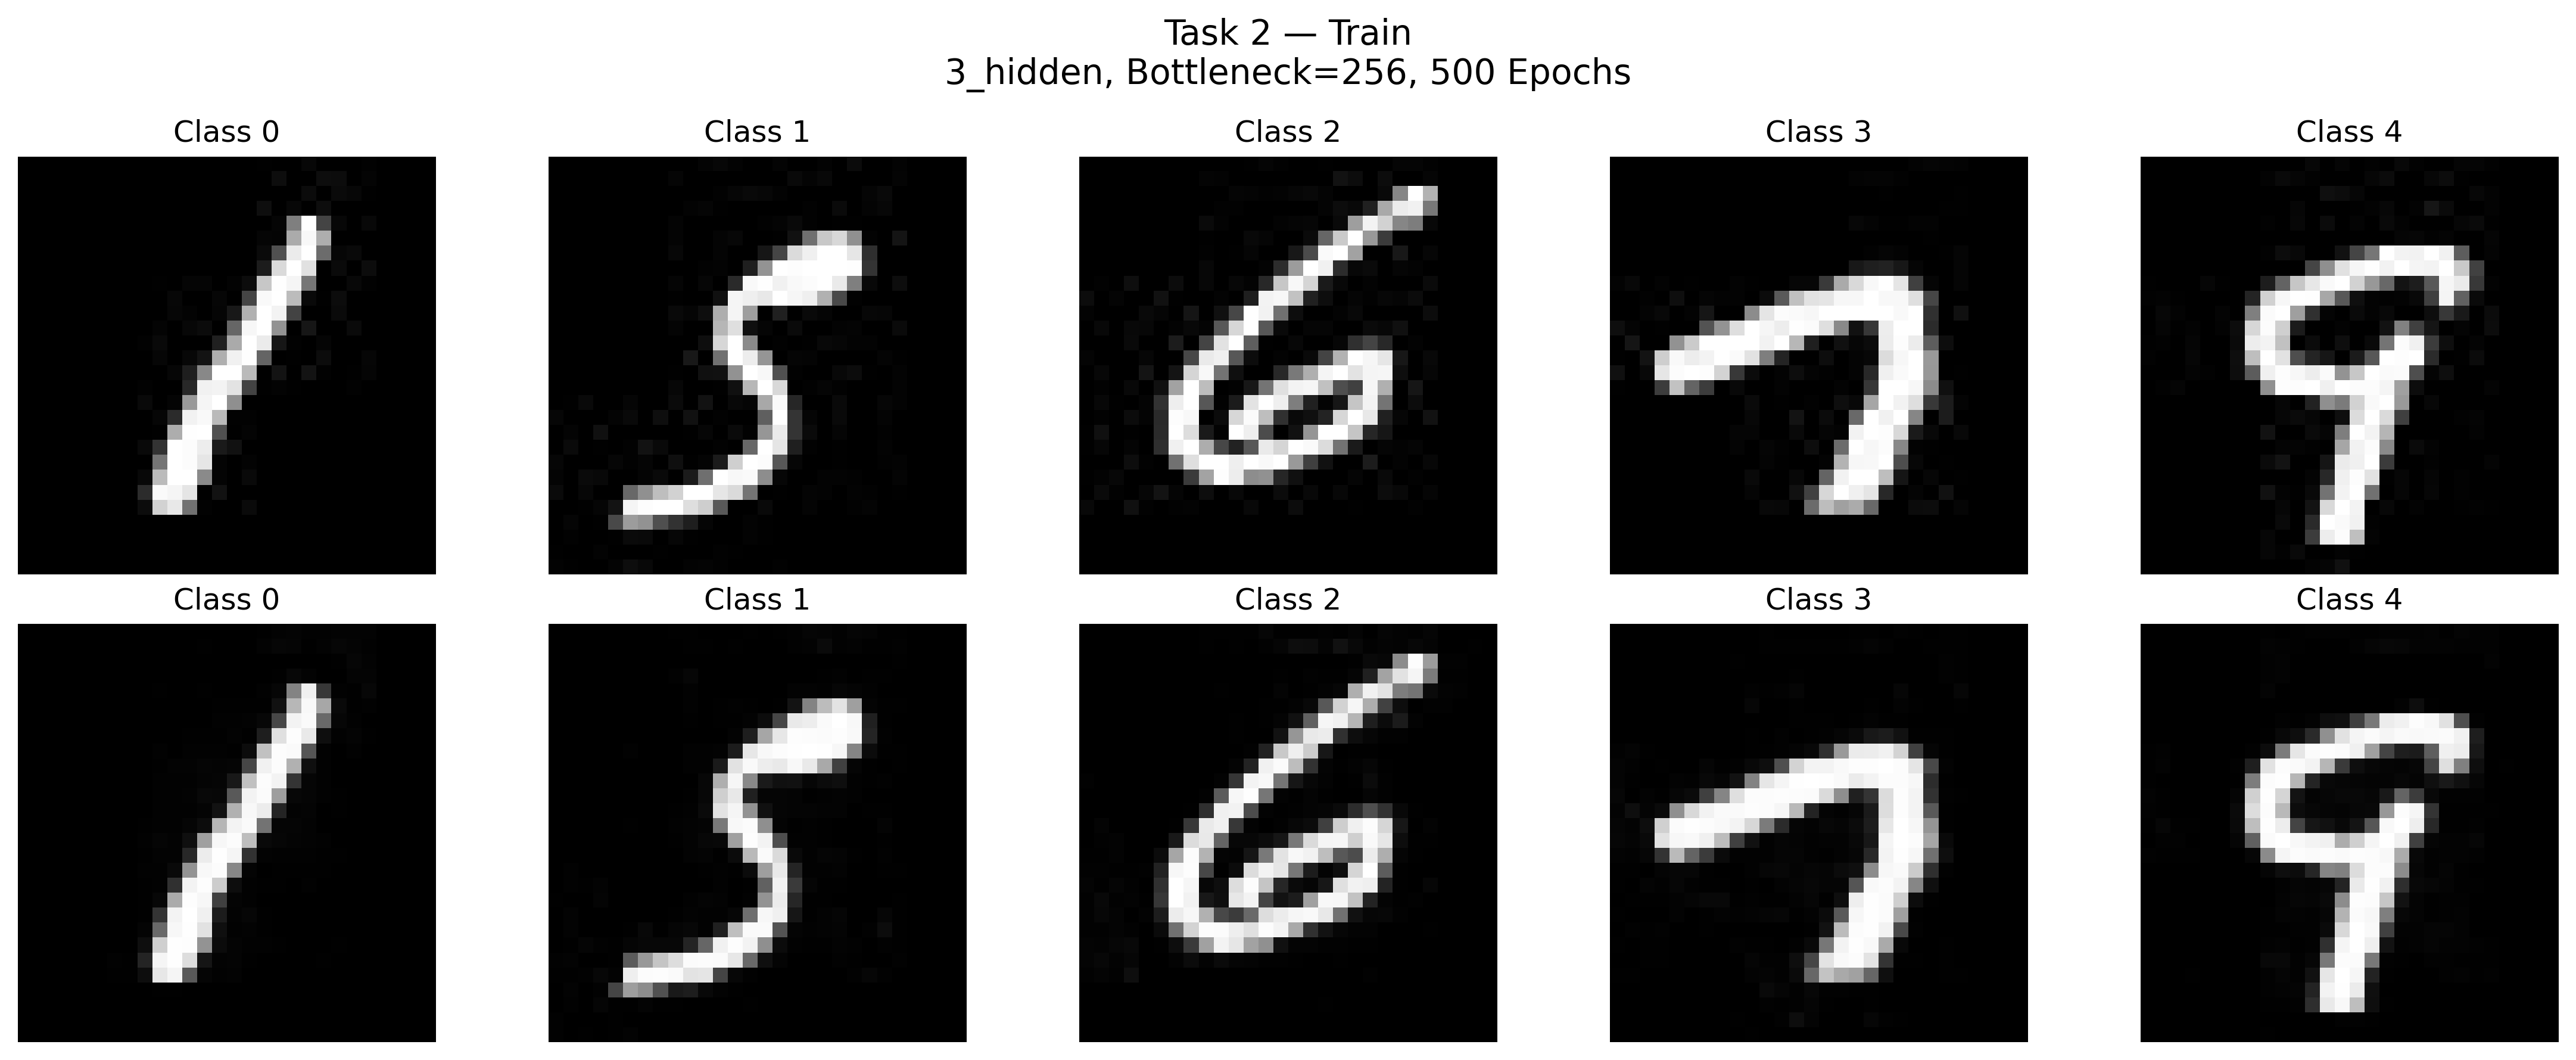
\includegraphics[width=0.96\linewidth,height=0.48\textheight,keepaspectratio]{figures/task2/model_reconstruction_visualization_500/train_3_hidden_bottleneck_256_500epochs.png}
\caption{Autoencoder reconstruction visualization: train 3 hidden with bottleneck of 256 neurons.}
\label{fig:task2_16}
\end{figure}

\begin{figure}[H]
\centering
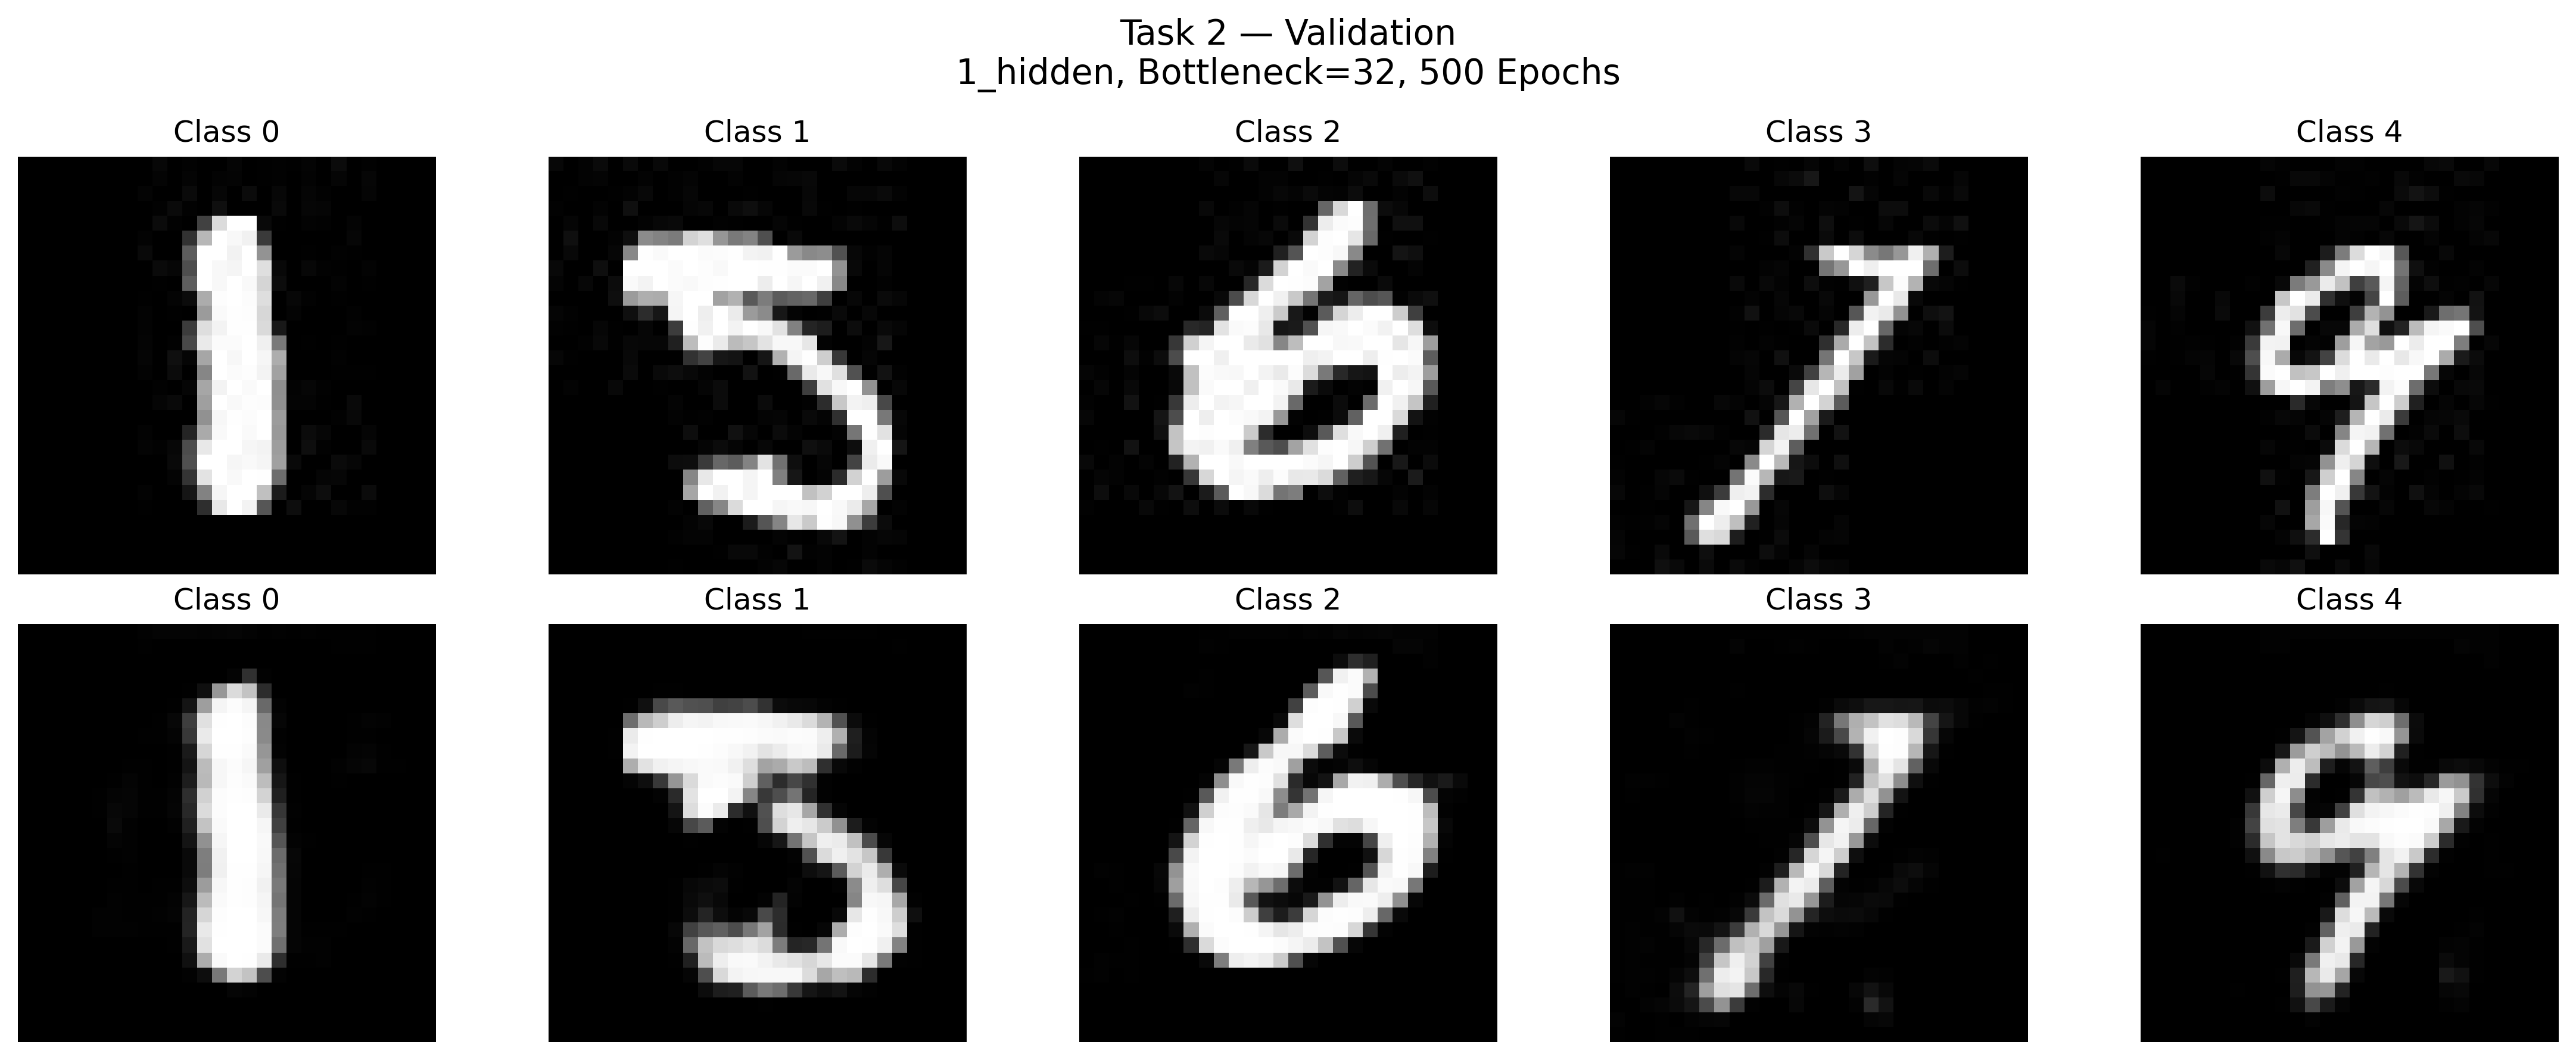
\includegraphics[width=0.96\linewidth,height=0.48\textheight,keepaspectratio]{figures/task2/model_reconstruction_visualization_500/validation_1_hidden_bottleneck_32_500epochs.png}
\caption{Autoencoder reconstruction visualization: validation 1 hidden with bottleneck of 32 neurons.}
\label{fig:task2_17}
\end{figure}

\begin{figure}[H]
\centering
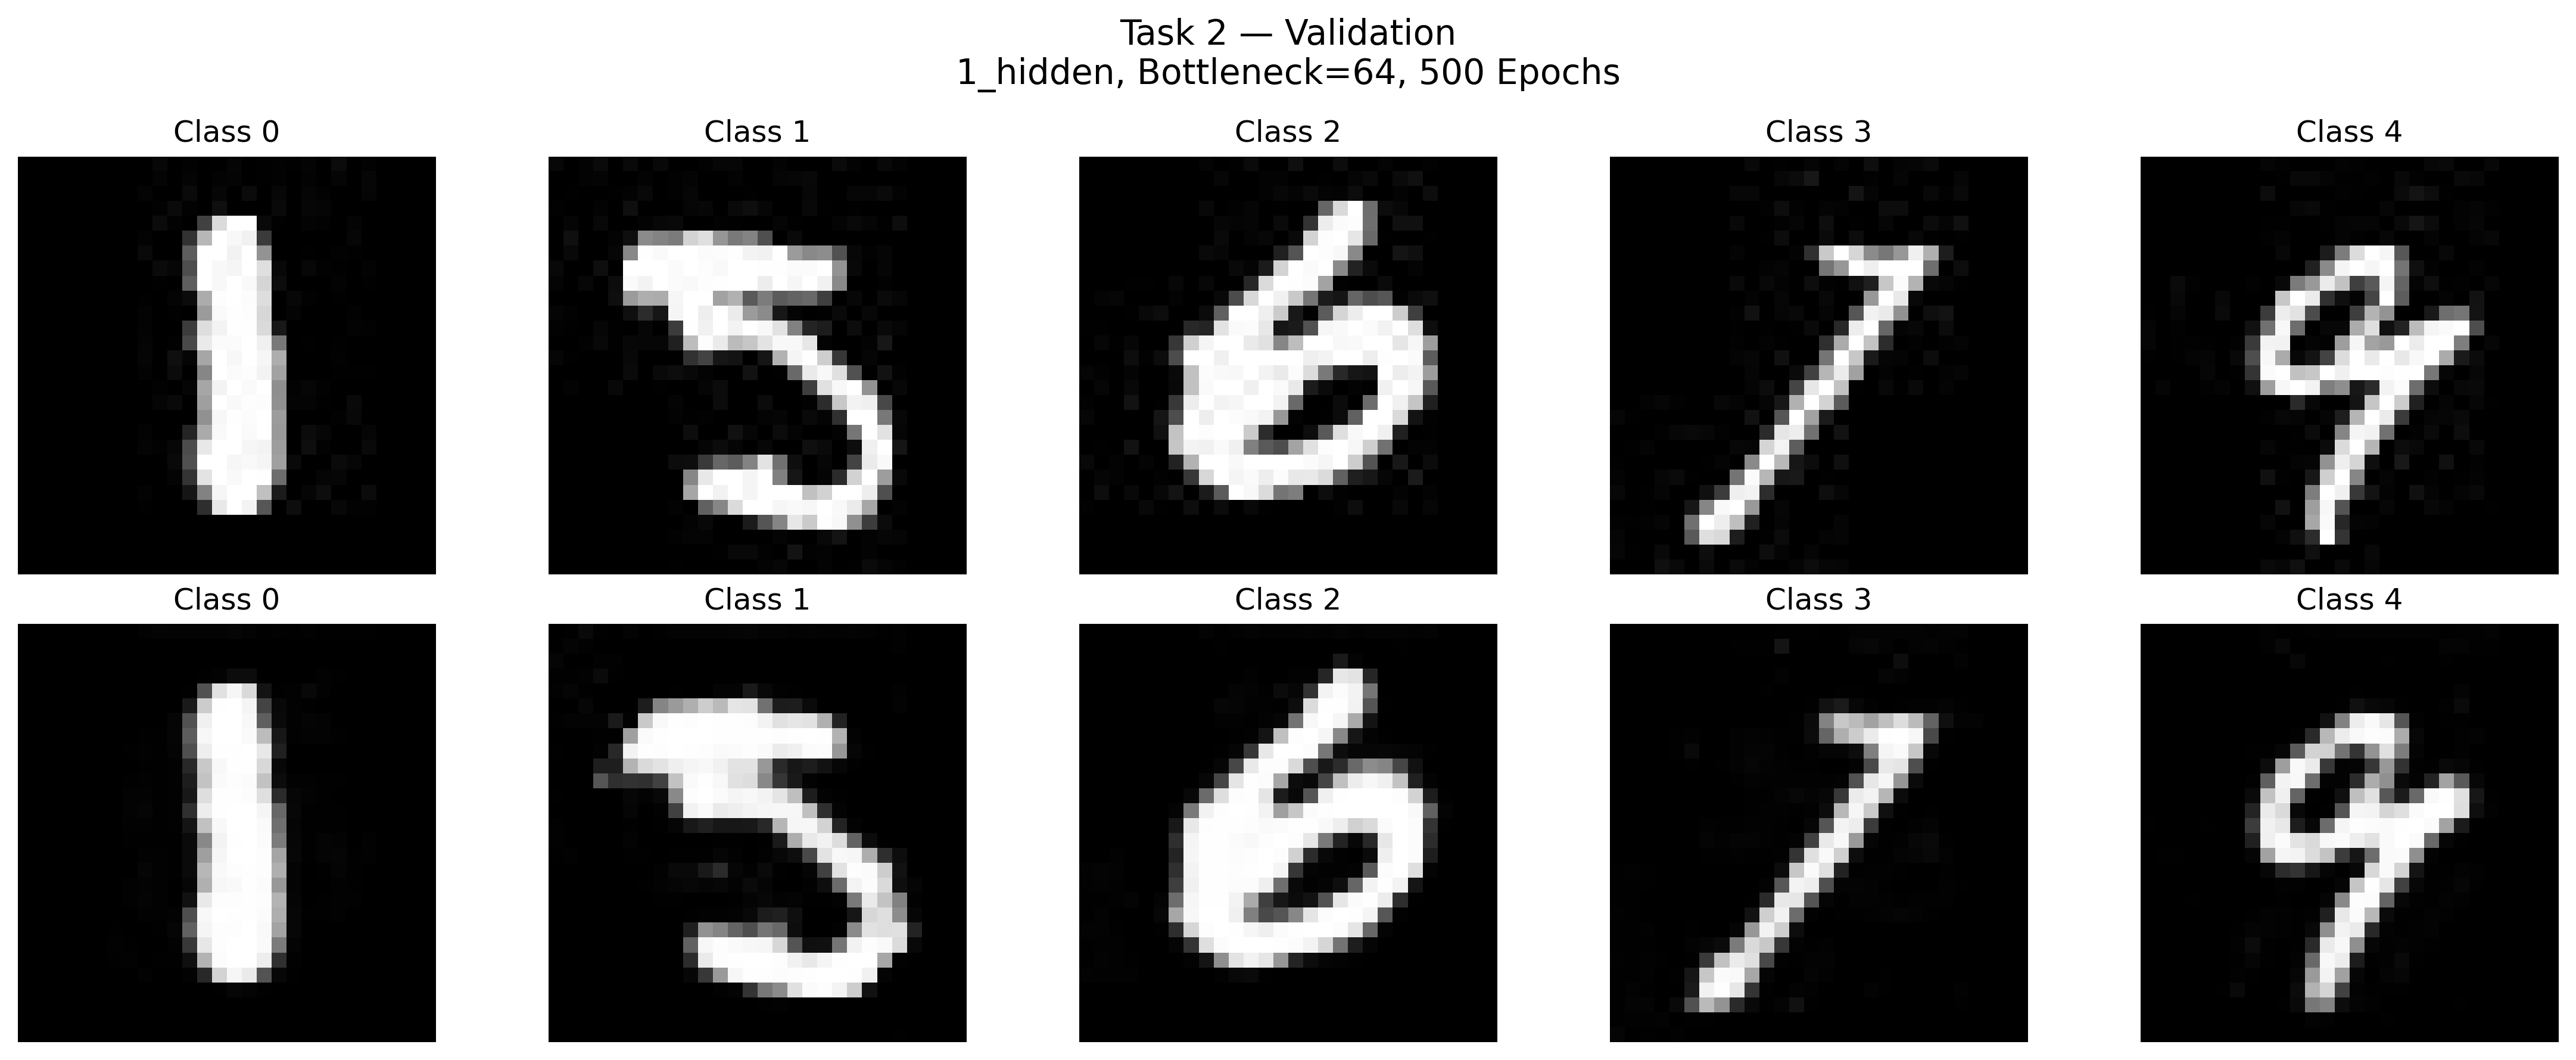
\includegraphics[width=0.96\linewidth,height=0.48\textheight,keepaspectratio]{figures/task2/model_reconstruction_visualization_500/validation_1_hidden_bottleneck_64_500epochs.png}
\caption{Autoencoder reconstruction visualization: validation 1 hidden with bottleneck of 64 neurons.}
\label{fig:task2_18}
\end{figure}

\begin{figure}[H]
\centering
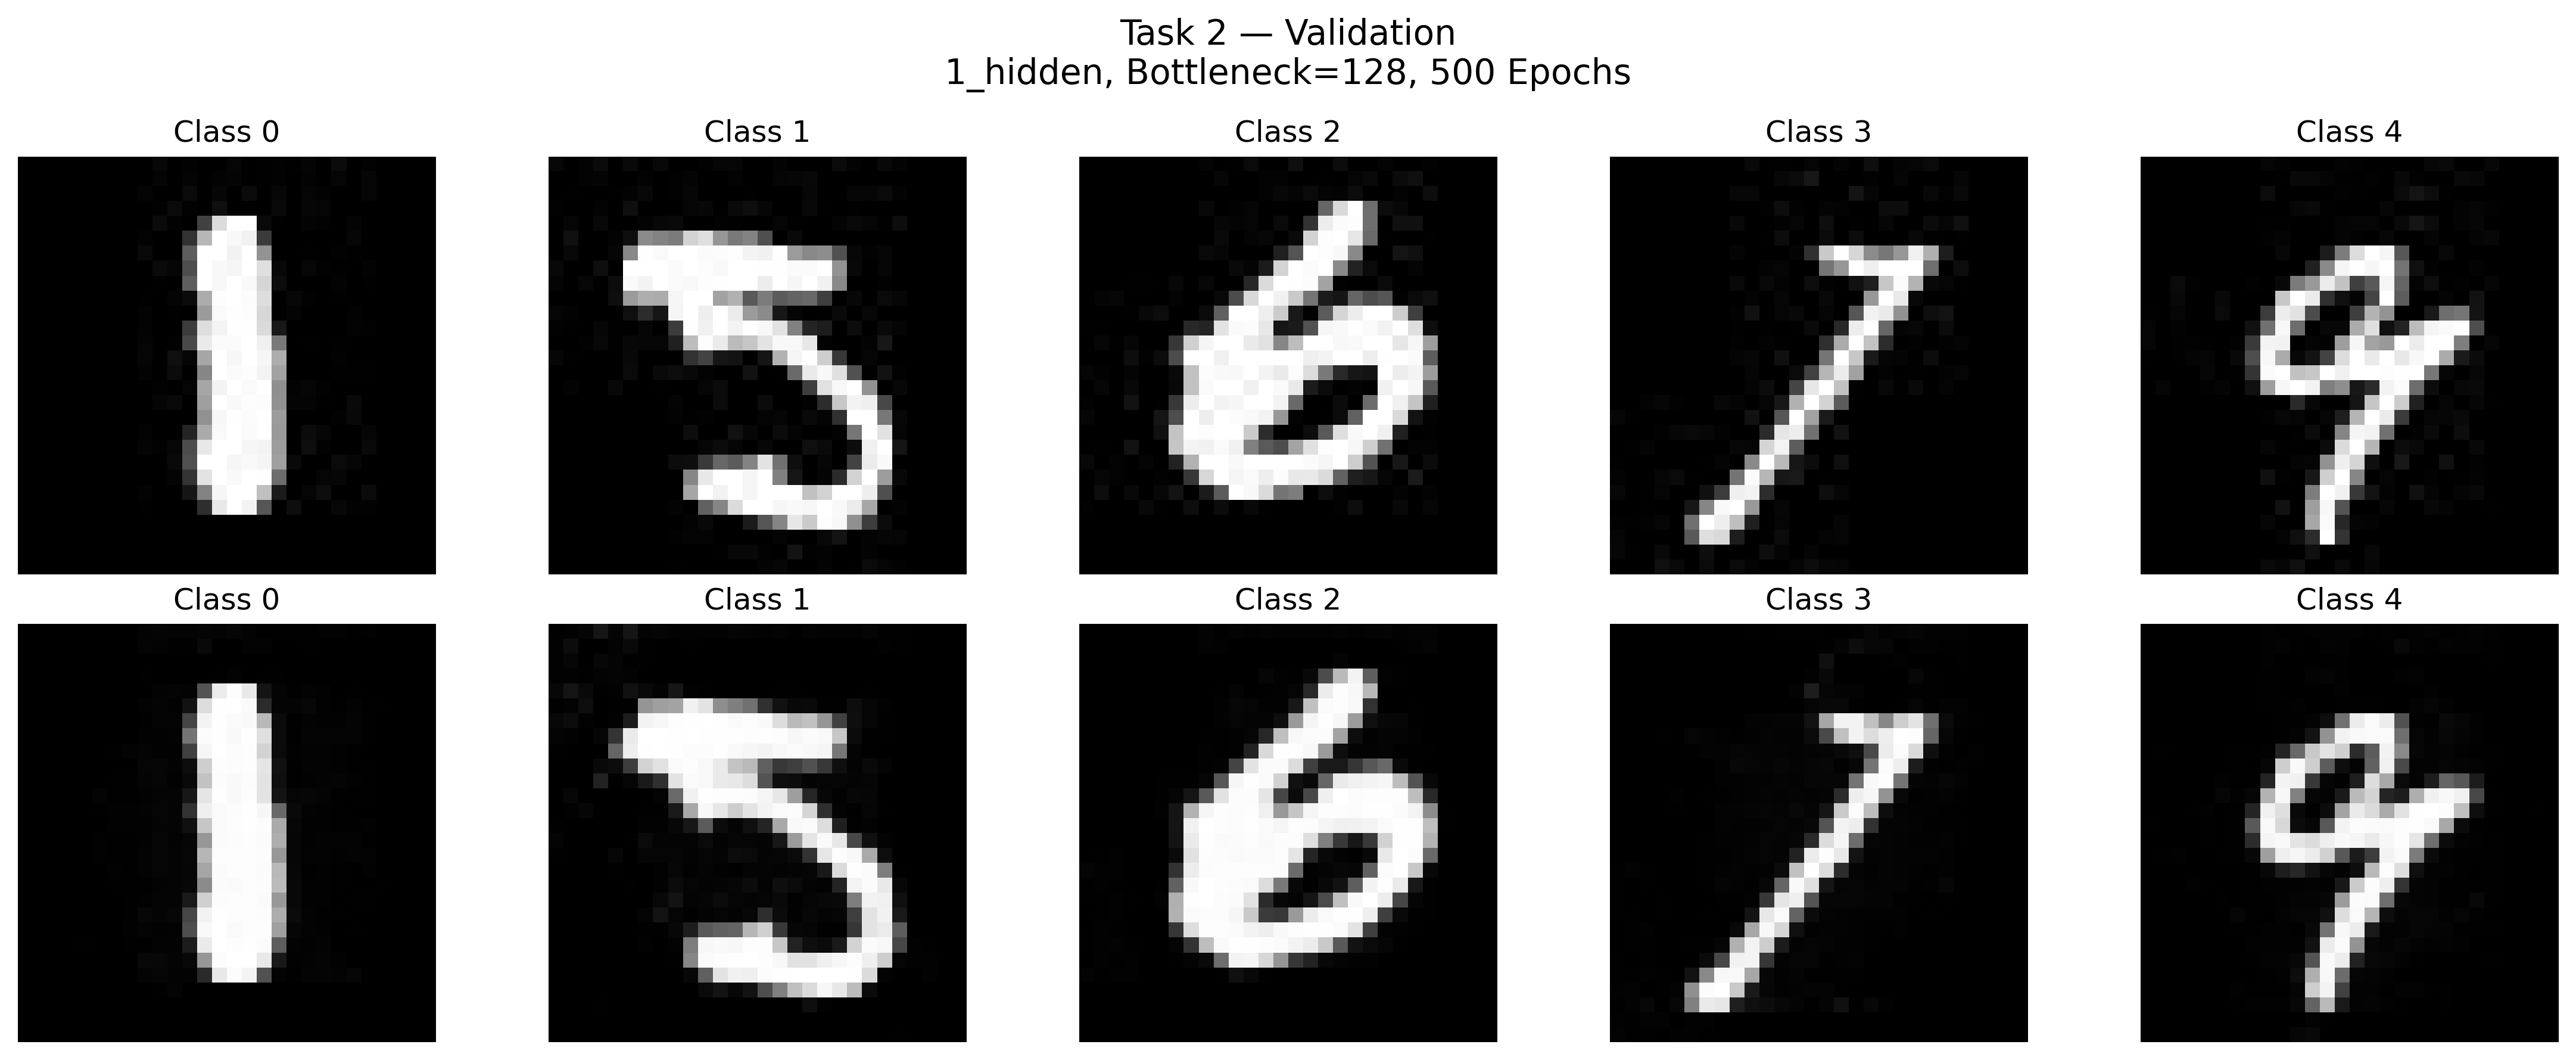
\includegraphics[width=0.96\linewidth,height=0.48\textheight,keepaspectratio]{figures/task2/model_reconstruction_visualization_500/validation_1_hidden_bottleneck_128_500epochs.png}
\caption{Autoencoder reconstruction visualization: validation 1 hidden with bottleneck of 128 neurons.}
\label{fig:task2_19}
\end{figure}

\begin{figure}[H]
\centering
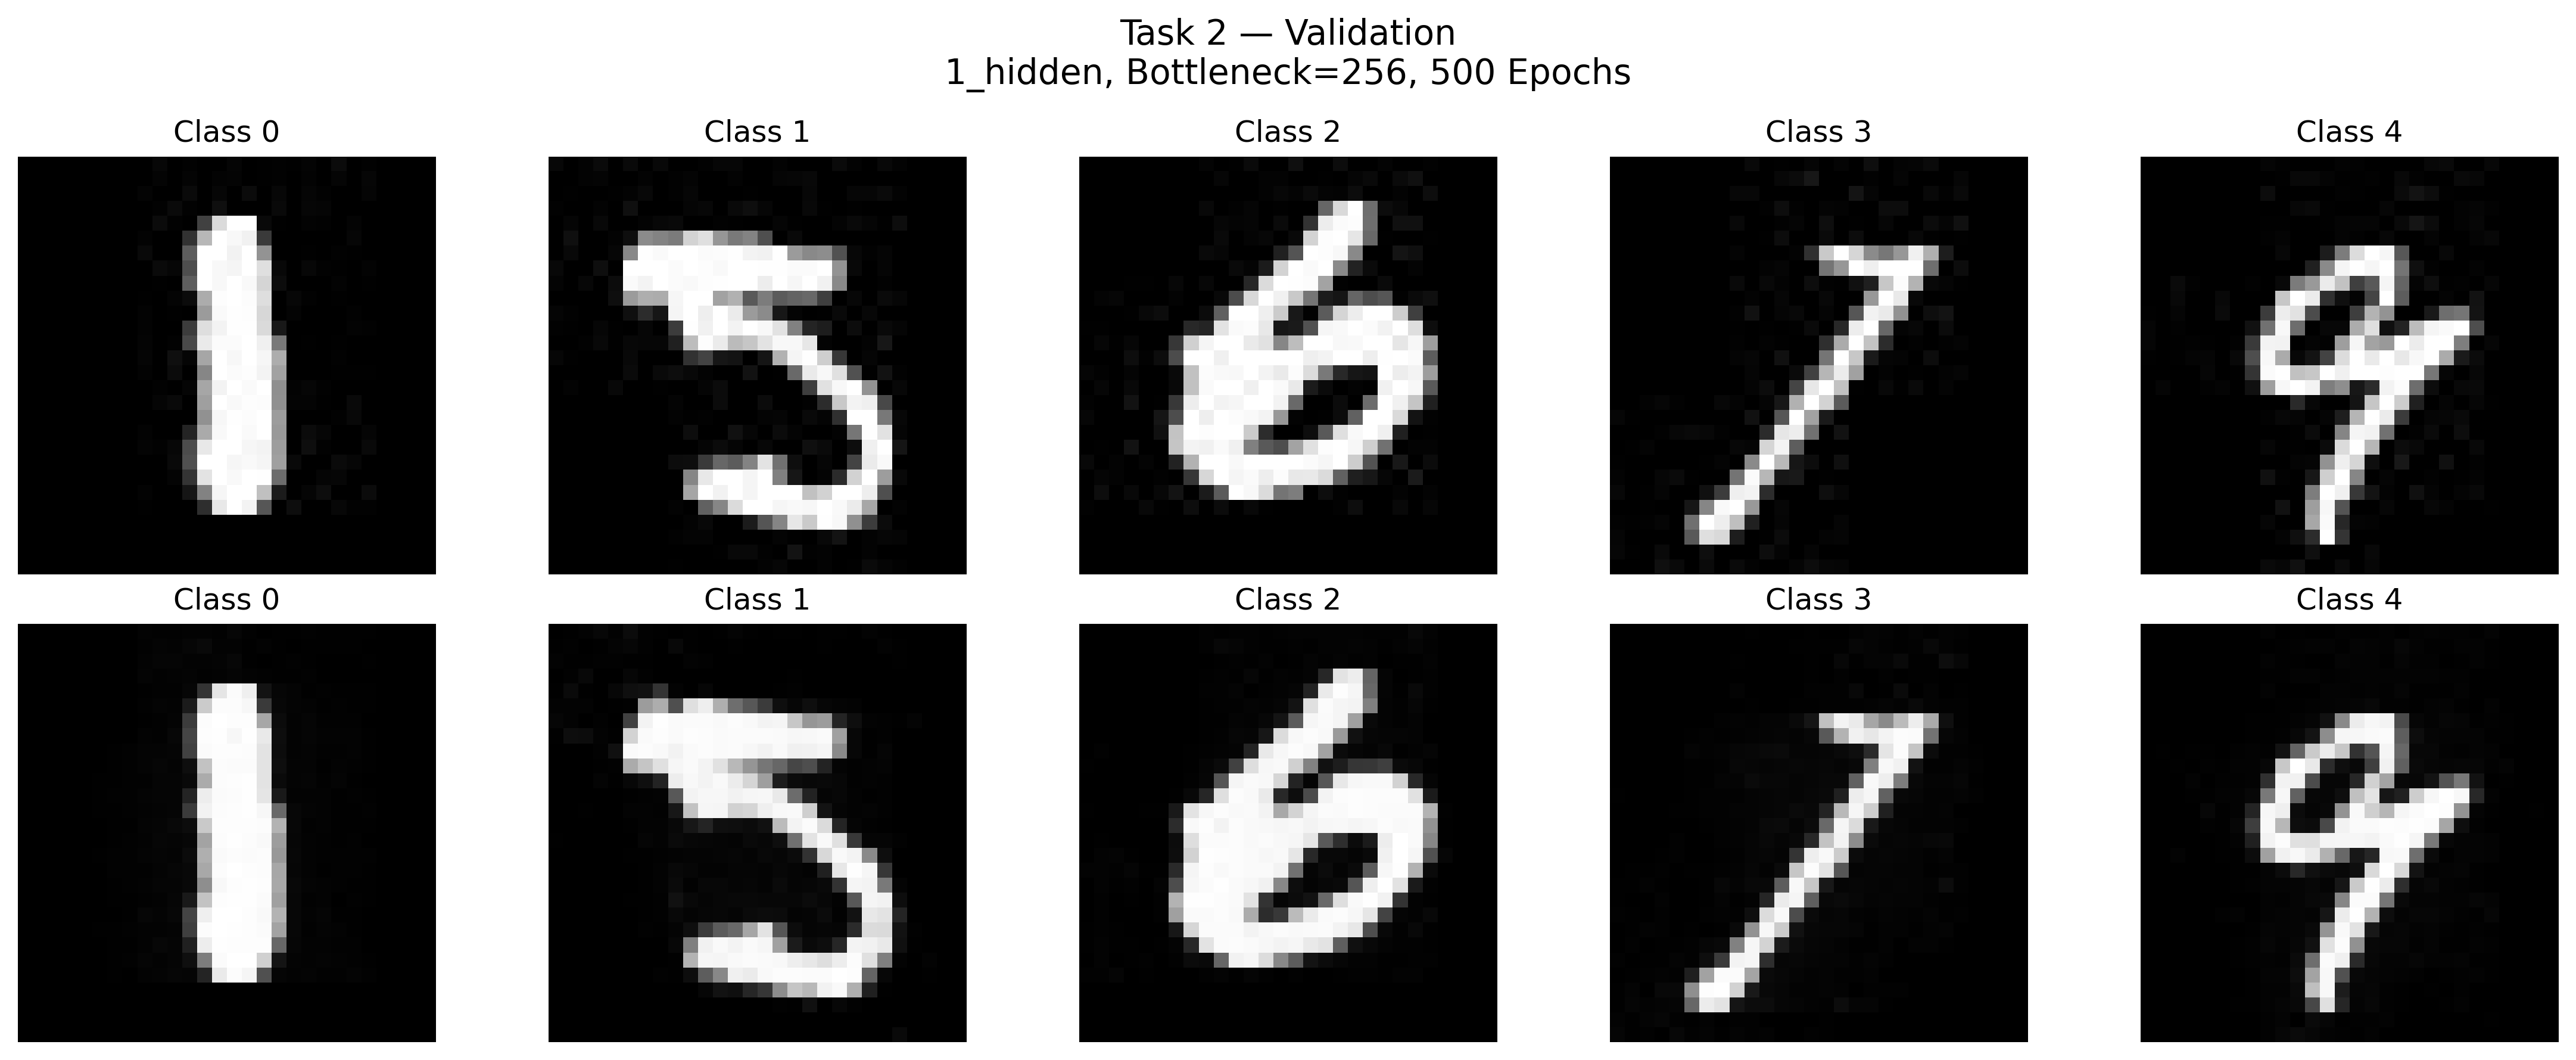
\includegraphics[width=0.96\linewidth,height=0.48\textheight,keepaspectratio]{figures/task2/model_reconstruction_visualization_500/validation_1_hidden_bottleneck_256_500epochs.png}
\caption{Autoencoder reconstruction visualization: validation 1 hidden with bottleneck of 256 neurons.}
\label{fig:task2_20}
\end{figure}

\begin{figure}[H]
\centering
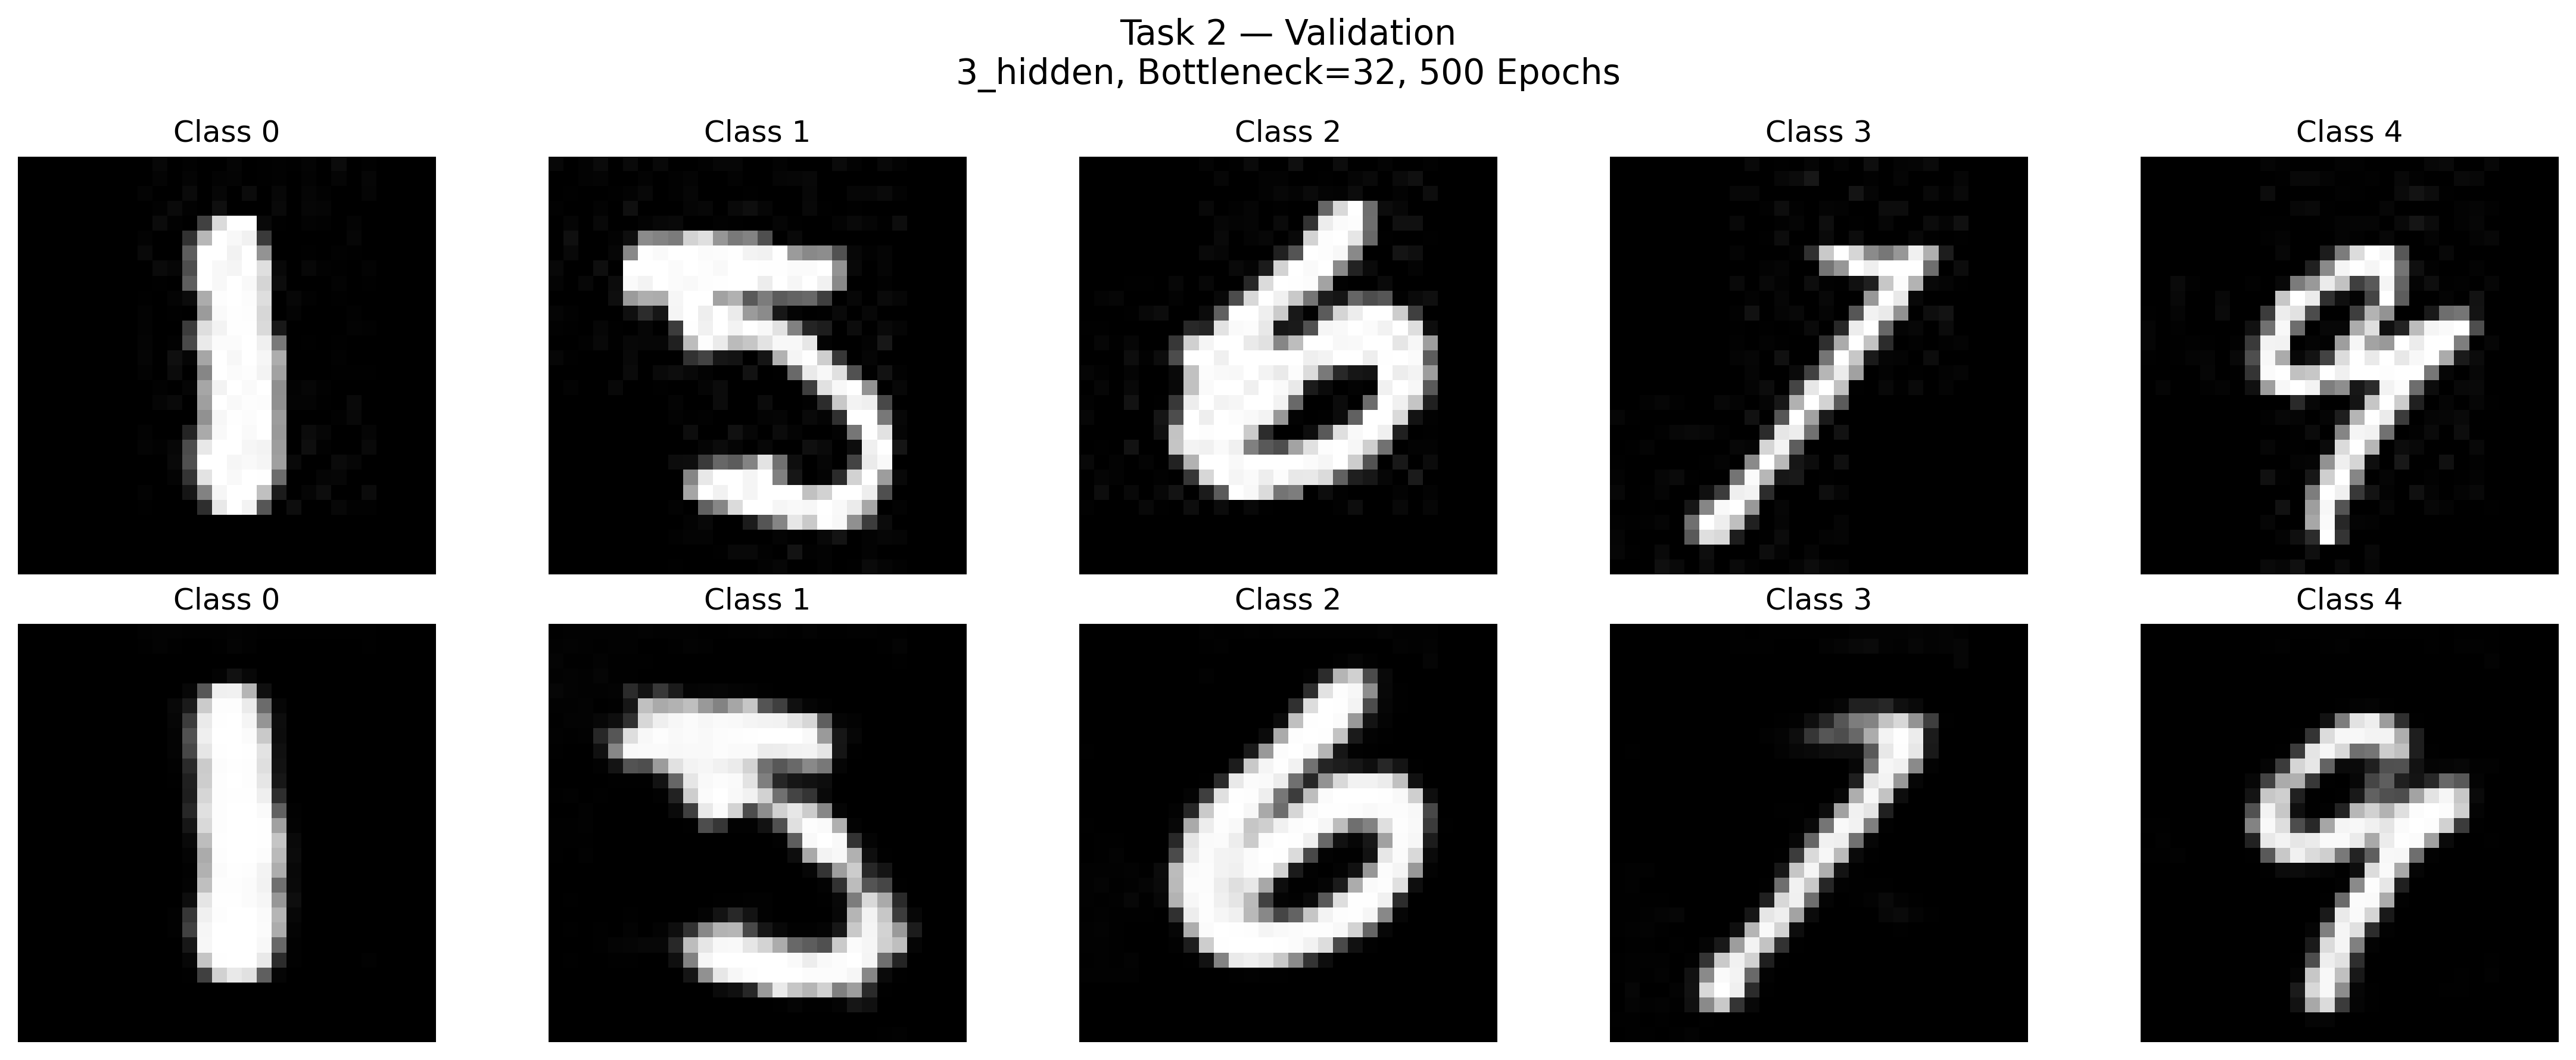
\includegraphics[width=0.96\linewidth,height=0.48\textheight,keepaspectratio]{figures/task2/model_reconstruction_visualization_500/validation_3_hidden_bottleneck_32_500epochs.png}
\caption{Autoencoder reconstruction visualization: validation 3 hidden with bottleneck of 32 neurons.}
\label{fig:task2_21}
\end{figure}

\begin{figure}[H]
\centering
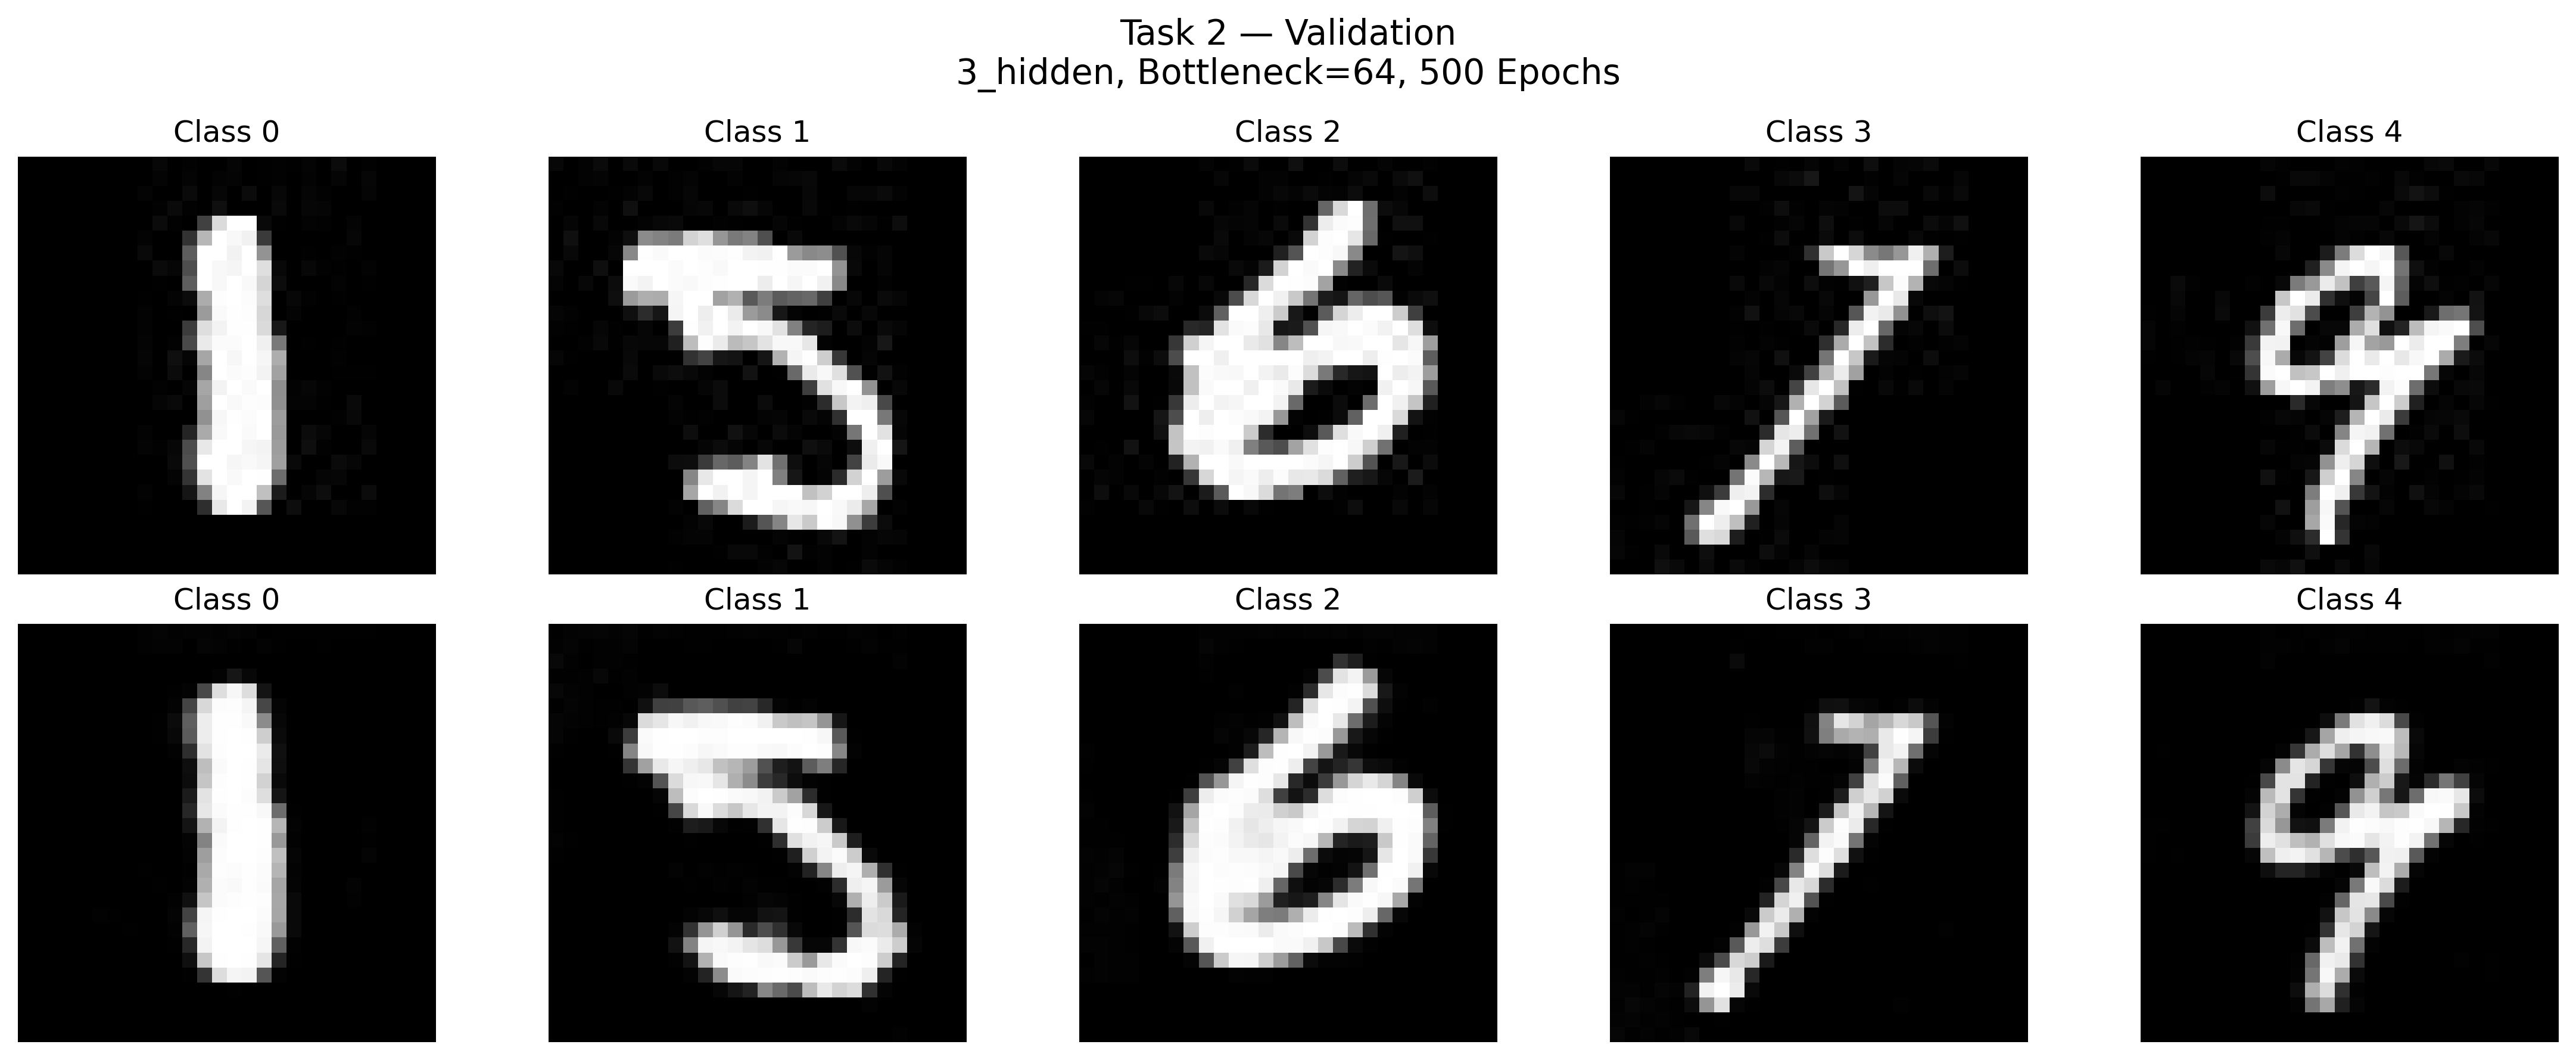
\includegraphics[width=0.96\linewidth,height=0.48\textheight,keepaspectratio]{figures/task2/model_reconstruction_visualization_500/validation_3_hidden_bottleneck_64_500epochs.png}
\caption{Autoencoder reconstruction visualization: validation 3 hidden with bottleneck of 64 neurons.}
\label{fig:task2_22}
\end{figure}

\begin{figure}[H]
\centering
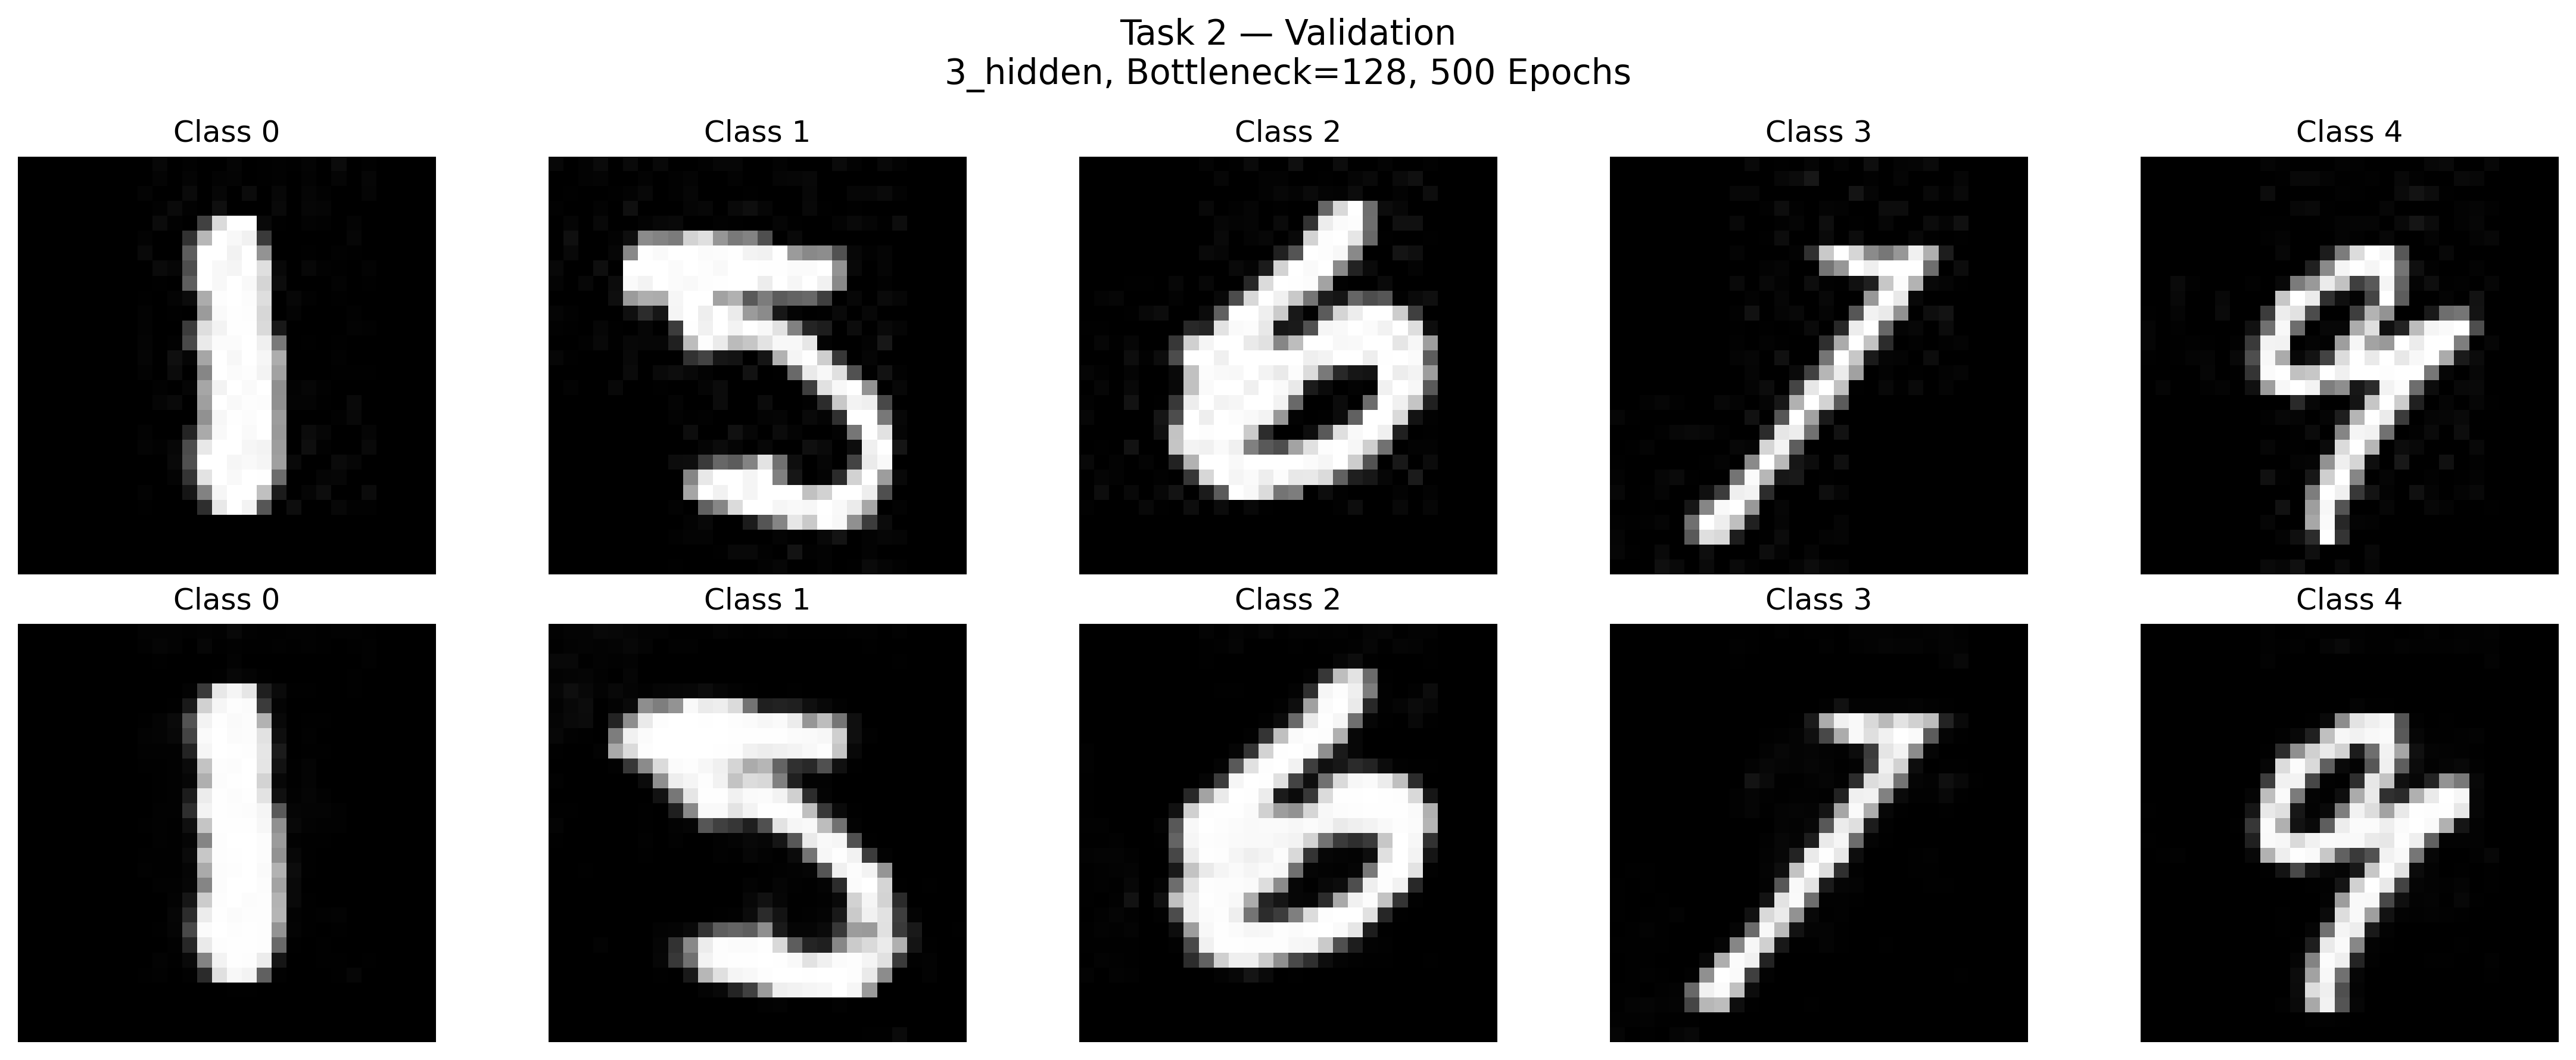
\includegraphics[width=0.96\linewidth,height=0.48\textheight,keepaspectratio]{figures/task2/model_reconstruction_visualization_500/validation_3_hidden_bottleneck_128_500epochs.png}
\caption{Autoencoder reconstruction visualization: validation 3 hidden with bottleneck of 128 neurons.}
\label{fig:task2_23}
\end{figure}

\begin{figure}[H]
\centering
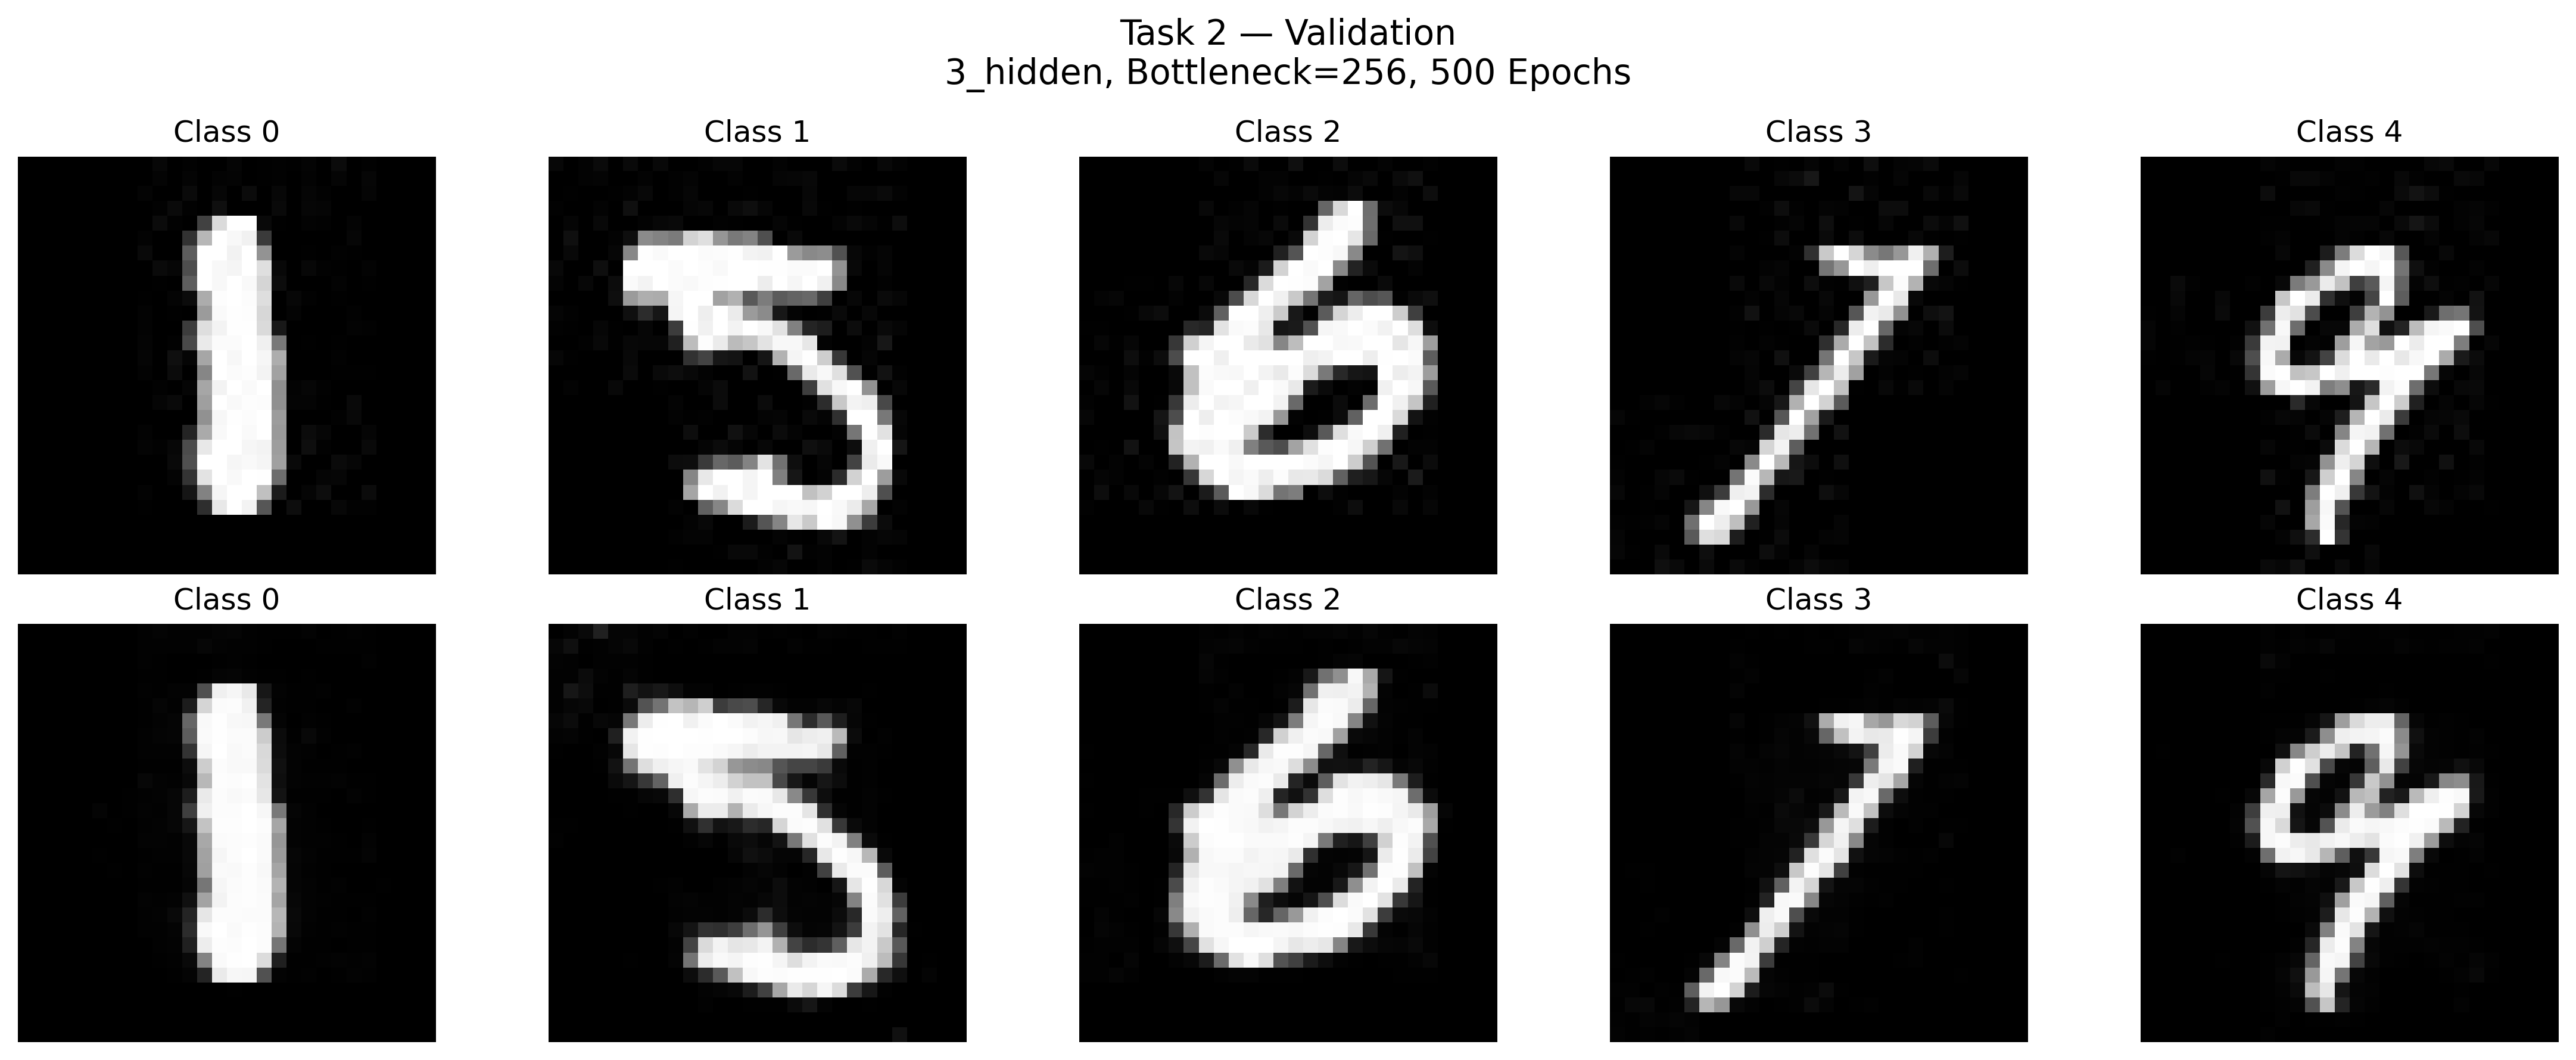
\includegraphics[width=0.96\linewidth,height=0.48\textheight,keepaspectratio]{figures/task2/model_reconstruction_visualization_500/validation_3_hidden_bottleneck_256_500epochs.png}
\caption{Autoencoder reconstruction visualization: validation 3 hidden with bottleneck of 256 neurons.}
\label{fig:task2_24}
\end{figure}
